\chapter{Revisão de Bibliográfica}
	\section{Conceitos utilizados}
	\label{ch:revisao}
		\subsection{Sinais digitais e sub-amostragem (\textit{downsampling})}
			\par Os sinais digitais, tanto de voz quanto aqueles vindos das medições de Eletroencefalograma (ECG), isto é, aqueles que estão amostrados e quantizados \cite{haykin2011sistemas}, constituem a base deste trabalho. Além do processo de digitalização, inerente ao ato de armazenar sinais em computadores, os mesmos podem sofrer, a depender da necessidade ou possibilidade, sub-amostragens ou \textit{downsamplings} \cite{robi2003}. Isso implica em uma estratégia de redução de dimensão e, comumente, ocorre após a conversão de domínio dos sinais com base em filtros digitais do tipo \textit{wavelet}, a serem apresentados adiante. Um exemplo consta na Figura \ref{fig:downsampling}, na qual as partes pretas contêm dados e as brancas representam os elementos removidos. Tendo em vista que este trabalho está baseado em sinais digitais de voz e ECG com base em \textit{wavelets}, o processo de sub-amostragem é essencial. 
			\begin{figure}[h]
				\centering
				\caption{Sub-amostragem}
				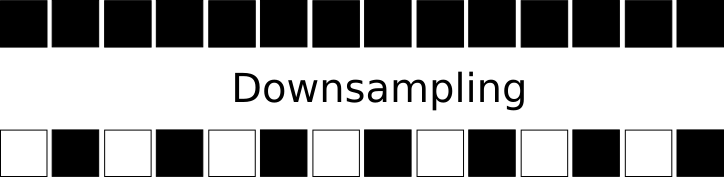
\includegraphics[width=0.4\linewidth]{images/downsampling}
				\label{fig:downsampling}
				\\Fonte: Elaborado pelo autor, 2023.
			\end{figure}
	
		\subsection{Caracterização dos processos de produção da voz humana}
			\par A fala possui três grandes áreas de estudo: A fisiológica, também conhecida como fonética articulatória, a acústica, referida como fonética acústica, e ainda, a perceptual, que cuida da percepção  da  fala \cite{kremer2014eficiencia}. Neste trabalho, o foco será apenas na questão acústica, pois não serão analisados aspectos da fisiologia relacionada à voz, mas sim os sinais sonoros propriamente ditos.
		
		\subsubsection{Sinais vozeados \textit{versus} não-vozeados}
			\par Quando da análise dos sinais de voz, consideram-se as partes vozeadas e não-vozeadas. Aquelas são produzidas com a ajuda da vibração quase periódica das pregas vocais, enquanto estas praticamente não contam com participação regrada da referida estrutura.
		
		\subsubsection{Frequência fundamental da voz}
			\par Também conhecida como $F_0$, é o componente periódico resultante da vibração das pregas vocais. Em termos de percepção, se pode interpretar $F_0$ como o tom da voz, isto é, a frequência de \textit{pitch} \cite{kremer2014eficiencia}. Vozes agudas tem uma frequência de \textit{pitch} alto, enquanto vozes mais graves tem baixa. A alteração da frequência (jitter) e/ou intensidade (shimmer) do \textit{pitch} durante a fala é definida como entonação,  porém, também pode indicar algum distúrbio ou doença relacionada ao trato vocal \cite{WERTZNER2005}.
			
			\par A frequência fundamental da voz é o número de vezes na qual uma forma de onda característica, que reflete a excitação pulmonar moldada pelas pregas vocais, se repete por unidade de tempo. Sendo assim, as medidas de $F_0$ geralmente são apresentadas em Hz \cite{freitas2013avaliaccao}.
			
			\par A medição de $F_0$ está sujeita a contaminações surgidas das variações naturais de \textit{pitch} típicas da voz humana \cite{freitas2013avaliaccao}. A importância de se medir $F_0$ corretamente vem do fato de que, além de carregar boa parte da informação da fala, ela é a base para construção das outras frequências que compõe os sinais de voz, que são múltiplas de $F_0$.
		
		\subsubsection{Formantes}
			\par O sinal de excitação que atravessa as pregas vocais é rico em harmônicas, isto é, frequências múltiplas da fundamental. Tais harmônicas podem ser atenuadas ou amplificadas, em função da estrutura dos tratos vocal e nasal de cada locutor. Particularmente, o primeiro formante ($F_1$), relaciona-se à  amplificação  sonora  na  cavidade  oral  posterior  e  à  posição  da  língua  no  plano  vertical;  o segundo  formante  ($F_2$)  à  cavidade  oral  anterior  e  à  posição  da  língua  no  plano  horizontal; o terceiro  formante  ($F_3$)  relaciona-se  às  cavidades  à  frente  e  atrás  do  ápice  da  língua e, finalmente,  o  quarto formante  ($F_4$) relaciona-se  ao  formato  da  laringe  e  da  faringe  na  mesma  altura  \cite{valencca2014analise}. Formantes caracterizam fortemente os locutores, pois cada indivíduo possui um formato de trato vocal e nasal. Assim, tais frequências, que podem ser capturadas com ferramentas diversas, a exemplo da Transformada \textit{Wavelet}, são de suma importância na área de verificação de locutores.
	
		\subsection{Escalas e energias dos sinais}
			\par A energia de um sinal digital $s[\cdot]$ com $M$ amostras é definida como
			
			\begin{equation}
				E = \sum\limits_{i=0}^{M-1}(s_i)^2 \qquad.   
			\end{equation}
			
			$E$ pode ainda sofrer normalizações e ter a sua mensuração restrita a uma parte específica do sinal sob análise. Possibilidades para tais restrições podem, por exemplo, envolver a escala BARK \cite{doi:10.1121-1.1908630} e MEL \cite{beranek1949acoustic} que serão utilizadas neste trabalho.
		\subsubsection{A escala BARK}
			\par BARK foi definida tendo em mente vários tipos de sinais acústicos. Essa escala corresponde ao conjunto de 25 bandas críticas da audição humana. Suas frequências-base de audiometria são, em Hz: \textbf{20, 100, 200, 300, 400, 510, 630, 770, 920, 1080, 1270, 1480, 1720, 2000, 2320, 2700, 3150, 3700, 4400, 5300, 6400, 7700, 9500, 12000, 15500}. Nessa escala,os sinais digitais no domínio temporal atravessam filtros passa-faixas \cite{bosi2002introduction} para os quais o início e o final da banda de passagem correspondem à frequências-base consecutivas resultando em um vetor de características com 24 coeficientes e, em seguida, as energias dos sinais filtrados são utilizadas como características descritivas de propriedades do sinal sob análise, como mostrado na Figura \ref{fig:barkfeaturevect}.
			\begin{figure}[h]
				\centering
				\caption{Cálculo de vetores de características com BARK}
				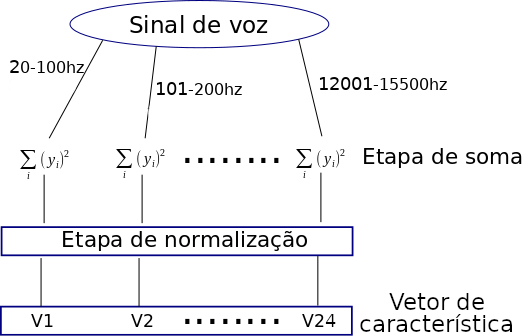
\includegraphics[width=0.6\linewidth]{images/barkFeatureVect}
				\label{fig:barkfeaturevect}
				\\Fonte: Elaborado pelo autor, 2023.
			\end{figure}
		\subsubsection{A escala MEL}
			\par Escala Mel, advinda do termo \textit{melody}, é uma adaptação da escala Bark para sinais de voz. Dentre as várias implementações de bandas críticas a escolhida foi a implementação que contém os valores em Hz: \textbf{20, 160, 394, 670, 1000, 1420, 1900, 2450, 3120, 4000, 5100, 6600, 9000, 14000}.
			
			\par A variante que será usada neste trabalho é conhecida como \textit{Mel-frequency cepstral coefficients}(MFCC) a qual inclui, além dos intervalos definidos, uma diminuição da correlação entre os componentes gerados via aplicação da Transformada Discreta Cosseno (DCT) \cite{salomon2007data} ou da Análise de Componentes Principais (PCA) \cite{jolliffe2006principal} seguida de duas derivações no vetor de características resultando em um total de 11 coeficientes. Nesse trabalho foi escolhida a DCT, no entanto, PCA poderia também ser escolhida sem prejuízos, o uso de uma ou outra depende da preferência do autor.
			
			\par Novamente, desconsiderando qualquer etapa intermediária que possa ser adicionada, as energias calculadas nos intervalos definidos na escala MEL podem, por si mesmas, constituir um vetor de características, como mostrado na Figura \ref{fig:barkfeaturevect}.
			
			\begin{figure}[h]
				\centering
				\caption{Cálculo de vetores de características com MEL}
				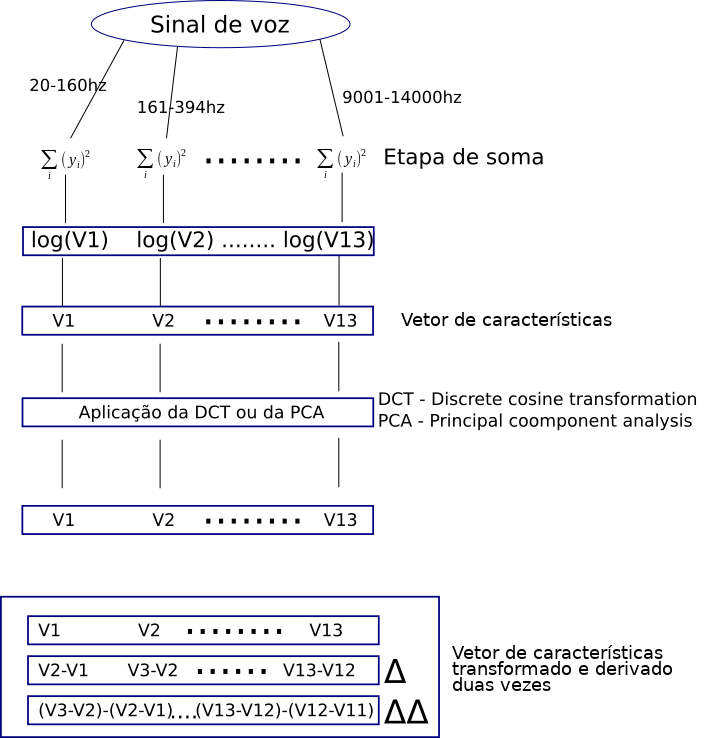
\includegraphics[width=0.8\linewidth]{images/melFeatureVect}
				\label{fig:melfeaturevect}
				\\Fonte: Elaborado pelo autor, 2023.
			\end{figure}
	
		\subsection{Filtros digitais \textit{wavelet}}
			\par Filtros digitais \textit{wavelet} têm sido utilizados com sucesso para suprir as deficiências de janelamento de sinal apresentadas pelas Transformadas de Fourier e de Fourier de Tempo Reduzido. \textit{Wavelets} contam com variadas funções-filtro e têm tamanho de janela variável, o que permite uma análise multirresolução \cite{Rod5254905}. Particularmente, as \textit{wavelets} proporcionam a análise do sinal de forma detalhada tanto no espectro de baixa frequência quanto no de alta contando com diferentes funções-base não periódicas diferentemente da tradicional transformada de Fourrier que utilizam somente as bases periódicas senoidal e cossenoidal.
			
			\par É importante observar que, quando se trata de Transformadas \textit{Wavelet}, seis elementos estão presentes: dois filtros de análise, dois filtros de síntese e as funções ortogonais \textit{scaling} e \textit{wavelet}. No tocante a sua aplicação, só a transformada direta, e não a inversa, será usada na construção dos vetores de características. Portanto, os filtros de síntese, a função \textit{scaling} e a função \textit{wavelet} não serão elementos abordados aqui: eles somente interessariam caso houvesse a necessidade da transformada inversa.
			
			\par No contexto dos filtros digitais baseados em \textit{wavelets}, o tamanho da janela recebe o nome de \textbf{suporte}. Janelas definem o tamanho do filtro que será aplicado ao sinal. Quando esse é pequeno (limitado), se diz que a janela tem \textbf{um suporte compacto} \cite{robi2003}.
			
			\par Se diz que uma \textit{wavelet} tem boa \textbf{resposta em frequência} quando, na aplicação da mesma para filtragem, não são causadas muitas pertubações indesejadas ao sinal, no domínio da frequência. Os filtros \textit{wavelet} de Daubechies \cite{daubechies1992ten} se destacam nesse quesito por serem \textit{maximamente planos} (\textit{maximally-flat}) \cite{butterworth1930} \cite{bianchi2007electronic} nos platôs de resposta em frequência como indicado na Figura \ref{fig:daubechies} ao contrário do que ocorre na Figura \ref{fig:nomaximallyflat}.
			
			\begin{figure}[h]
				\centering
				\caption{Platôs maximamente planos em um filtro digital: característica da família de Daubechies}
				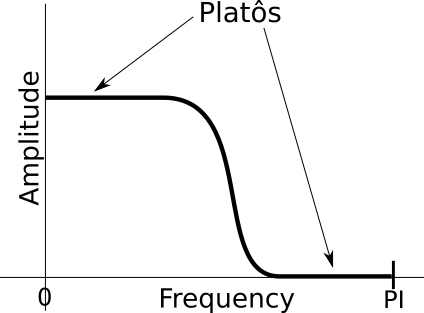
\includegraphics[width=0.3\linewidth]{images/daubechies}
				\label{fig:daubechies}
				\\Fonte: Elaborado pelo autor, 2023.
			\end{figure}
			
			\begin{figure}[h]
				\centering
				\caption{Platôs não maximamente planos de um filtro digital: características de outros filtros \textit{wavelet}, distintos da família de Daubechies}
				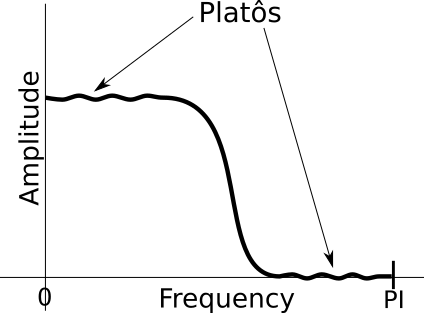
\includegraphics[width=0.3\linewidth]{images/noMaximallyFlat}
				\label{fig:nomaximallyflat}
				\\Fonte: Elaborado pelo autor, 2023.
			\end{figure}
			
			\par Além da resposta em frequência, na aplicação de um filtro digital \textit{wavelet} também é possível considerar a \textbf{resposta em fase}, que constitui um atraso ou adiantamento do sinal filtrado em relação ao sinal original, ambos no domínio temporal. Esse deslocamento pode ser \textbf{linear}, \textbf{quase linear} ou \textbf{não linear}: 
	
			\begin{itemize}
				\item na resposta em fase \textbf{linear}, há o mesmo deslocamento de fase para todos os componentes do sinal;
				\item quando a resposta em fase é \textbf{quase linear} existe uma pequena diferença no deslocamento dos diferentes componentes do sinal;
				\item finalmente, quando a resposta é \textbf{não linear}, acontece um deslocamento significativamente heterogêneo para as diferentes frequências que compõe o sinal.
			\end{itemize}
			
			\par Idealmente, é desejável que todo filtro apresente boa resposta em frequência e em fase linear. Características de fase e frequência de algumas famílias de filtros \textit{wavelet} constam na Tabela \ref{tab:waveletsProperties}.
			
			\begin{table}[h]
	\centering
	\caption{Algumas das \textit{wavelets} mais usadas e suas propriedades}
	\begin{tabular}{|c|p{75mm}|c|}
			\hline 
			\textbf{Wavelet} & \textbf{Resposta em frequência} & \textbf{Resposta em fase} \\ 
			\hline 
			Haar & Pobre &  Linear \\ 
			\hline 
			Daubechies & mais próxima da ideal à medida que o \newline  suporte aumenta; \textit{maximally-flat}  &  Não linear \\ 
			\hline 
			Symmlets & mais próxima da ideal à medida que o \newline  suporte aumenta; não \textit{maximally-flat}  & Quase linear \\ 
			\hline 
			Coiflets & mais próxima da ideal à medida que o \newline  suporte aumenta; não \textit{maximally-flat}  & Quase linear \\ 
			\hline 
	\end{tabular} 
	\label{tab:waveletsProperties}
	\\Fonte: Elaborado pelo autor, 2022.
\end{table}

	
		\subsubsection{O algoritmo de Mallat para a Transformada \textit{Wavelet}}
			\par Baseando-se no artigo \cite{7079589}, percebe-se que algoritmo de Mallat faz com que aplicação das \textit{wavelets} seja uma simples multiplicação de matrizes. O sinal que deve ser transformado se torna uma matriz linear vertical. Os filtros passa-baixa e passa-alta tornam-se, nessa ordem, linhas de uma matriz quadrada que será completada segundo regras que serão mostradas mais adiante. É importante que essa matriz quadrada tenha a mesma dimensão que o sinal a ser transformado.
			
			\par Interessantemente, para que seja possível a transformação \textit{wavelet}, basta ter disponível o vetor do filtro passa-baixas calculado a partir da \textit{mother wavelet}, que é a função geradora desse filtro, já que o passa-alta pode ser construído a partindo-se da ortogonalidade do primeiro.
			
			\par Determinar a ortogonal de um vetor significa construir um vetor, tal que, o produto escalar do vetor original com sua respectiva ortogonal seja nulo.
			
			\par Considerando $h[\cdot]$ como sendo o vetor do filtro passa-baixas e $g[\cdot]$ seu correspondente ortogonal, tem-se que $h[\cdot] \cdot g[\cdot] = 0 \qquad .$
			\par Portanto, se $h[\cdot]=[a, b, c, d]$ então seu ortogonal será $g[\cdot]=[d, -c, b, -a]$ pois:
			$$
			h[\cdot] \cdot g[\cdot]  =  [a, b, c, d] \cdot [d, -c, b, -a] = (a \cdot d) + (b \cdot (-c)) + (c \cdot b) + (d \cdot (-a)) = ad - ad + bc - bc = 0 \qquad.
			$$
	
			\par A título de exemplo, considera-se:
			\begin{itemize}
				\item o filtro passa baixa baseado na \textit{wavelet} Haar: $h[\cdot] = [\frac{1}{\sqrt{2}}, \frac{1}{\sqrt{2}}]$
				\item o seu respectivo vetor ortogonal: $g[\cdot] = [\frac{1}{\sqrt{2}}, \frac{-1}{\sqrt{2}}]$
				\item e também o seguinte sinal-exemplo de entrada: $s = \{1,2,3,4\}$
			\end{itemize}
			
			\par Se o tamanho do sinal a ser tratado é quatro e se pretende-se aplicar o filtro Haar, a seguinte matriz de coeficientes é construída:
			\begin{equation}
				\begin{pmatrix}
					\frac{1}{\sqrt{2}}, \frac{1}{\sqrt{2}}, 0, 0\\
					\frac{1}{\sqrt{2}}, \frac{-1}{\sqrt{2}}, 0, 0\\
					0, 0, \frac{1}{\sqrt{2}}, \frac{1}{\sqrt{2}}\\
					0, 0, \frac{1}{\sqrt{2}}, \frac{1}{\sqrt{2}}
					\label{eq:haarFilters}
				\end{pmatrix} 
			\end{equation}
		
			\par Tendo em vista que a dimensão do sinal sob análise é diferente da dimensão do filtro, basta completar cada uma das linhas da matriz de coeficientes com zeros. A matriz é montada de forma que ela seja ortogonal.
			
			\par Montada a matriz de filtros, segue-se com os cálculos da transformada:
			\begin{equation}
				\begin{pmatrix}
					\frac{1}{\sqrt{2}}, \frac{1}{\sqrt{2}}, 0, 0\\
					\frac{1}{\sqrt{2}}, \frac{-1}{\sqrt{2}}, 0, 0\\
					0, 0, \frac{1}{\sqrt{2}}, \frac{1}{\sqrt{2}}\\
					0, 0, \frac{1}{\sqrt{2}}, \frac{1}{\sqrt{2}}\\
				\end{pmatrix} 
				\cdot
				\begin{pmatrix}
					1\\
					2\\
					3\\
					4\\
				\end{pmatrix} 
				=
				\begin{pmatrix}
					\frac{3}{\sqrt{2}}\\
					\frac{-1}{\sqrt{2}}\\
					\frac{7}{\sqrt{2}}\\
					\frac{-1}{\sqrt{2}}
				\end{pmatrix}
				\label{eq:haarMultiplic}
			\end{equation}

			\par Realizada a multiplicação, é necessário montar o sinal filtrado. Isso é feito escolhendo, dentro do resultado, valores alternadamente de forma que o vetor resultante seja:
			
			\begin{equation}
				resultado = \Big[
				\frac{3}{\sqrt{2}},
				\frac{7}{\sqrt{2}},
				\frac{-1}{\sqrt{2}},
				\frac{-1}{\sqrt{2}}
				\Big]\qquad.
				\label{eq:haarResult}
			\end{equation}
			
			\par Percebe-se que, na transformação descrita nas Equações \ref{eq:haarFilters}, \ref{eq:haarMultiplic} e \ref{eq:haarResult}, a \textbf{aplicação dos filtros sobre o vetor de entrada ocorreu apenas uma vez}. Sendo assim, se diz que o sinal recebeu uma \textbf{transformação de nível 1}. A cada transformação, há uma separação do sinal em dois componentes: o de baixa e o de alta frequência.
	
			\par Embora haja um limite, que será mencionado adiante, é possível aplicar mais de um nível de decomposição ao sinal. Para que se possa fazer isso, a Transformada \textit{Wavelet} nível 2 deve considerar apenas a parte de baixas frequências da primeira transformada; a transformada de nível 3 deve considerar apenas a parte de baixas frequências da transformada nível 2, e assim consecutivamente.
			
			\par Nos exemplos numéricos mostrados nas Tabelas \ref{tab:regularWaveletExample}, \ref{tab:packetWaveletExampleLF} e \ref{tab:packetWaveletExampleHF}, usou-se um filtro normalizado cujos coeficientes são $\{\dfrac{1}{2},-\dfrac{1}{2}\}$. Os dados destacados em \textbf{verde} correspondem ao \textbf{vetor original} que será tratado. Cada uma das linhas são os resultados das transformações nos níveis 1, 2, 3 e 4, respectivamente. As partes em \textbf{azul} correspondem à porção de \textbf{baixas frequências}, enquanto que as partes em \textbf{amarelo} correspondem às porções de \textbf{altas frequências}.
			
			\par Percebe-se que na Tabela \ref{tab:regularWaveletExample}, a partir da transformação nível 2, apenas as partes de baixa frequência são modificadas. Isso implica que, no momento da implementação do algoritmo de Mallat \textbf{para níveis maiores que 1}, a abordagem será \textbf{recursiva}. Em outras palavras, a partir do nível 1 se deve aplicar Mallat apenas às porções de baixas-frequências geradas pela transformação anterior.
	
			\begin{table}[h]
	\fontsize{9}{\baselineskip} \selectfont
	\newcommand{\mc}[3]{\multicolumn{#1}{#2}{#3}}
	\definecolor{tcA}{rgb}{0.65098,0.65098,0.65098}
	\definecolor{tcD}{rgb}{1,0.94902,0}
	\definecolor{tcC}{rgb}{0,0.5,1}
	\definecolor{tcB}{rgb}{0.447059,0.74902,0.266667}
	\begin{center}
		\caption[Exemplo numérico da transformação \textit{wavelet}]{Exemplo numérico da transformação \textit{wavelet} aplicada a um vetor. Tabela completa no \autoref{sec:aplicaWavelet}.}
		\begin{tabular}{c|ccccccccccccccc|c}
			% use packages: color,colortbl
			\mc{1}{>{\columncolor{tcA}}c|}{\textbf{Sinal}} & \mc{1}{>{\columncolor{tcB}}c}{\textbf{32}} & \mc{1}{>{\columncolor{tcB}}c}{\textbf{10}} & \mc{1}{>{\columncolor{tcB}}c}{\textbf{20}} & \mc{1}{>{\columncolor{tcB}}c}{\textbf{38}} & \mc{1}{>{\columncolor{tcB}}c}{\textbf{37}} & \mc{1}{>{\columncolor{tcB}}c}{\textbf{28}} & \mc{1}{>{\columncolor{tcB}}c}{\textbf{38}} & \mc{1}{>{\columncolor{tcB}}c}{\textbf{34}} & \mc{1}{>{\columncolor{tcB}}c}{\textbf{18}} & \mc{1}{>{\columncolor{tcB}}c}{\textbf{24}} & \mc{1}{>{\columncolor{tcB}}c}{\textbf{24}} & \mc{1}{>{\columncolor{tcB}}c}{\textbf{9}} & \mc{1}{>{\columncolor{tcB}}c}{\textbf{23}} & \mc{1}{>{\columncolor{tcB}}c}{\textbf{24}} & \mc{1}{>{\columncolor{tcB}}c}{\textbf{28}} & \mc{1}{>{\columncolor{tcB}}c}{\textbf{34}}\\
			\hline
			
			\mc{1}{>{\columncolor{tcA}}c|}{Nível 01} & \mc{1}{>{\columncolor{tcC}}c}{21} & \mc{1}{>{\columncolor{tcC}}c}{29} & \mc{1}{>{\columncolor{tcC}}c}{32,5} & \mc{1}{>{\columncolor{tcC}}c}{36} & \mc{1}{>{\columncolor{tcC}}c}{21} & \mc{1}{>{\columncolor{tcC}}c}{16,5} & \mc{1}{>{\columncolor{tcC}}c}{23,5} & \mc{1}{>{\columncolor{tcC}}c}{31} & \mc{1}{>{\columncolor{tcD}}c}{11} & \mc{1}{>{\columncolor{tcD}}c}{-9} & \mc{1}{>{\columncolor{tcD}}c}{4,5} & \mc{1}{>{\columncolor{tcD}}c}{2} & \mc{1}{>{\columncolor{tcD}}c}{-3} & \mc{1}{>{\columncolor{tcD}}c}{7,5} & \mc{1}{>{\columncolor{tcD}}c}{-0,5} & \mc{1}{>{\columncolor{tcD}}c}{-3}\\
			\hline
			
			\mc{1}{>{\columncolor{tcA}}c|}{Nível 02} & \mc{1}{>{\columncolor{tcC}}c}{25} & \mc{1}{>{\columncolor{tcC}}c}{34,25} & \mc{1}{>{\columncolor{tcC}}c}{18,75} & \mc{1}{>{\columncolor{tcC}}c}{27,25} & \mc{1}{>{\columncolor{tcD}}c}{-4} & \mc{1}{>{\columncolor{tcD}}c}{-1,75} & \mc{1}{>{\columncolor{tcD}}c}{2,25} & \mc{1}{>{\columncolor{tcD}}c}{-3,75} & \mc{1}{>{\columncolor{tcD}}c}{11} & \mc{1}{>{\columncolor{tcD}}c}{-9} & \mc{1}{>{\columncolor{tcD}}c}{4,5} & \mc{1}{>{\columncolor{tcD}}c}{2} & \mc{1}{>{\columncolor{tcD}}c}{-3} & \mc{1}{>{\columncolor{tcD}}c}{7,5} & \mc{1}{>{\columncolor{tcD}}c}{-0,5} & \mc{1}{>{\columncolor{tcD}}c}{-3}\\
			\hline
			
			\mc{1}{>{\columncolor{tcA}}c|}{Nível 03} & \mc{1}{>{\columncolor{tcC}}c}{29,62} & \mc{1}{>{\columncolor{tcC}}c}{23} & \mc{1}{>{\columncolor{tcD}}c}{-4,625} & \mc{1}{>{\columncolor{tcD}}c}{-4,25} & \mc{1}{>{\columncolor{tcD}}c}{-4} & \mc{1}{>{\columncolor{tcD}}c}{-1,75} & \mc{1}{>{\columncolor{tcD}}c}{2,25} & \mc{1}{>{\columncolor{tcD}}c}{-3,75} & \mc{1}{>{\columncolor{tcD}}c}{11} & \mc{1}{>{\columncolor{tcD}}c}{-9} & \mc{1}{>{\columncolor{tcD}}c}{4,5} & \mc{1}{>{\columncolor{tcD}}c}{2} & \mc{1}{>{\columncolor{tcD}}c}{-3} & \mc{1}{>{\columncolor{tcD}}c}{7,5} & \mc{1}{>{\columncolor{tcD}}c}{-0,5} & \mc{1}{>{\columncolor{tcD}}c}{-3}\\
			\hline
			
			\mc{1}{>{\columncolor{tcA}}c|}{Nível 04} & \mc{1}{>{\columncolor{tcC}}c}{26,3125} & \mc{1}{>{\columncolor{tcD}}c}{3,3125} & \mc{1}{>{\columncolor{tcD}}c}{-4,625} & \mc{1}{>{\columncolor{tcD}}c}{-4,25} & \mc{1}{>{\columncolor{tcD}}c}{-4} & \mc{1}{>{\columncolor{tcD}}c}{-1,75} & \mc{1}{>{\columncolor{tcD}}c}{2,25} & \mc{1}{>{\columncolor{tcD}}c}{-3,75} & \mc{1}{>{\columncolor{tcD}}c}{11} & \mc{1}{>{\columncolor{tcD}}c}{-9} & \mc{1}{>{\columncolor{tcD}}c}{4,5} & \mc{1}{>{\columncolor{tcD}}c}{2} & \mc{1}{>{\columncolor{tcD}}c}{-3} & \mc{1}{>{\columncolor{tcD}}c}{7,5} & \mc{1}{>{\columncolor{tcD}}c}{-0,5} & \mc{1}{>{\columncolor{tcD}}c}{-3}
		\end{tabular}
		\label{tab:regularWaveletExample}
		\fontsize{12}{\baselineskip} \selectfont
		\\Fonte: Elaborado pelo autor, 2022.
	\end{center}
\end{table}
	
		\subsubsection{O algoritmo de Mallat e a Transformada \textit{Wavelet-Packet}}
			\par Na Transformada \textit{Wavelet-Packet}, os filtros aplicados são os mesmos da Transformada \textit{Wavelet} e o procedimento recursivo de cálculo também é o mesmo, no entanto, realizada a transformação de nível 1, a transformada de nível 2 deve ser aplicada aos componentes de baixa e de alta frequência. Sendo assim a Transformada \textit{Wavelet-Packet} obtém um nível de detalhes em todo o espectro de frequência, maior do que uma transformação regular. 
			
			\par Os exemplos mostrados nas Tabelas \ref{tab:packetWaveletExampleLF} e \ref{tab:packetWaveletExampleHF} permitem perceber como se dão as transformações na porção de \textbf{baixa} e de \textbf{alta} frequências, respectivamente, após a transformação \textit{wavelet-packet} de nível 1, 2, 3 e 4.
			
			\par Devido ao \textit{downsampling} aplicado às porções de alta frequência, essas partes acabam por ficar ``espelhadas'' no espectro \cite{Jensen_2001}, ou seja, suas sequências ficam invertidas. Para resolver esse problema e preservar a ordem das sub-bandas no sinal transformado, os filtros são aplicados em ordem inversa nas porções de alta frequência. Isso altera como o algoritmo de Mallat deve ser implementado para a Transformada \textit{Wavelet-Packet}, já que dessa vez é preciso se atentar a ordem da aplicação dos filtros passa-alta e passa-baixa.
	
			\begin{table}[h]
	\newcommand{\mc}[3]{\multicolumn{#1}{#2}{#3}}
	\definecolor{tcA}{rgb}{0.65098,0.65098,0.65098}
	\definecolor{tcD}{rgb}{1,0.94902,0}
	\definecolor{tcC}{rgb}{0,0.5,1}
	\definecolor{tcB}{rgb}{0.447059,0.74902,0.266667}
	\begin{center}
		\caption{Exemplo numérico de \textit{wavelet-packet} Haar aplicada ao vetor da Tabela \ref{tab:regularWaveletExample} (porção das baixas frequências)}
		\begin{tabular}{l|llllllll|}
			% use packages: color,colortbl
			\mc{1}{>{\columncolor{tcA}}l|}{\textbf{Sinal}} & \mc{1}{>{\columncolor{tcB}}l}{\textbf{32}} & \mc{1}{>{\columncolor{tcB}}l}{\textbf{10}} & \mc{1}{>{\columncolor{tcB}}l}{\textbf{20}} & \mc{1}{>{\columncolor{tcB}}l}{\textbf{38}} & \mc{1}{>{\columncolor{tcB}}l}{\textbf{37}} & \mc{1}{>{\columncolor{tcB}}l}{\textbf{28}} & \mc{1}{>{\columncolor{tcB}}l}{\textbf{38}} & \mc{1}{>{\columncolor{tcB}}l|}{\textbf{34}}\\
			\hline
			
			\mc{1}{>{\columncolor{tcA}}l|}{Nivel 01} & \mc{1}{>{\columncolor{tcC}}l}{21} & \mc{1}{>{\columncolor{tcC}}l}{29} & \mc{1}{>{\columncolor{tcC}}l}{32,5} & \mc{1}{>{\columncolor{tcC}}l}{36} & \mc{1}{>{\columncolor{tcC}}l}{21} & \mc{1}{>{\columncolor{tcC}}l}{16,5} & \mc{1}{>{\columncolor{tcC}}l}{23,5} & \mc{1}{>{\columncolor{tcC}}l|}{31}\\
			\hline
			
			\mc{1}{>{\columncolor{tcA}}l|}{Nivel 02} & \mc{1}{>{\columncolor{tcC}}l}{25} & \mc{1}{>{\columncolor{tcC}}l}{34,25} & \mc{1}{>{\columncolor{tcC}}l}{18,75} & \mc{1}{>{\columncolor{tcC}}l|}{27,25} & \mc{1}{>{\columncolor{tcD}}l}{-4} & \mc{1}{>{\columncolor{tcD}}l}{-1,75} & \mc{1}{>{\columncolor{tcD}}l}{2,25} & \mc{1}{>{\columncolor{tcD}}l|}{-3,75}\\
			\hline
			
			\mc{1}{>{\columncolor{tcA}}l|}{Nivel 03} & \mc{1}{>{\columncolor{tcC}}l}{29,62} & \mc{1}{>{\columncolor{tcC}}l|}{23} & \mc{1}{>{\columncolor{tcD}}l}{-4,625} & \mc{1}{>{\columncolor{tcD}}l|}{-4,25} & \mc{1}{>{\columncolor{tcD}}l}{-1,125} & \mc{1}{>{\columncolor{tcD}}l|}{3} & \mc{1}{>{\columncolor{tcC}}l}{-2,875} & \mc{1}{>{\columncolor{tcC}}l|}{-0,75}\\
			\hline
			
			\mc{1}{>{\columncolor{tcA}}l|}{Nivel 04} & \mc{1}{>{\columncolor{tcC}}l|}{26,3125} & \mc{1}{>{\columncolor{tcD}}l|}{3,3125} & \mc{1}{>{\columncolor{tcD}}l|}{-0,1875} & \mc{1}{>{\columncolor{tcC}}l|}{-4,4375} & \mc{1}{>{\columncolor{tcC}}l|}{0,9375} & \mc{1}{>{\columncolor{tcD}}l|}{-2,0625} & \mc{1}{>{\columncolor{tcD}}l|}{-1,0625} & \mc{1}{>{\columncolor{tcC}}l|}{-1,8125}\\
		\end{tabular}
		\label{tab:packetWaveletExampleLF}
		\\Fonte: Elaborado pelo autor, 2023.
	\end{center}
\end{table}

\begin{table}[h]
	\newcommand{\mc}[3]{\multicolumn{#1}{#2}{#3}}
	\definecolor{tcA}{rgb}{0.65098,0.65098,0.65098}
	\definecolor{tcC}{rgb}{1,0.94902,0}
	\definecolor{tcD}{rgb}{0,0.5,1}
	\definecolor{tcB}{rgb}{0.447059,0.74902,0.266667}
	\begin{center}
		\caption{Exemplo numérico de \textit{wavelet-packet} Haar aplicada ao vetor da Tabela \ref{tab:regularWaveletExample} (porção das altas frequências)}
		\begin{tabular}{c|cccccccc}
			% use packages: color,colortbl
			\mc{1}{>{\columncolor{tcA}}c|}{\textbf{Sinal}} & \mc{1}{>{\columncolor{tcB}}c}{\textbf{18}} & \mc{1}{>{\columncolor{tcB}}c}{\textbf{24}} & \mc{1}{>{\columncolor{tcB}}c}{\textbf{24}} & \mc{1}{>{\columncolor{tcB}}c}{\textbf{9}} & \mc{1}{>{\columncolor{tcB}}c}{\textbf{23}} & \mc{1}{>{\columncolor{tcB}}c}{\textbf{24}} & \mc{1}{>{\columncolor{tcB}}c}{\textbf{28}} & \mc{1}{>{\columncolor{tcB}}c|}{\textbf{34}}\\\hline
			\mc{1}{>{\columncolor{tcA}}c|}{Nivel 01} & \mc{1}{>{\columncolor{tcC}}c}{11} & \mc{1}{>{\columncolor{tcC}}c}{-9} & \mc{1}{>{\columncolor{tcC}}c}{4,5} & \mc{1}{>{\columncolor{tcC}}c}{2} & \mc{1}{>{\columncolor{tcC}}c}{-3} & \mc{1}{>{\columncolor{tcC}}c}{7,5} & \mc{1}{>{\columncolor{tcC}}c}{-0,5} & \mc{1}{>{\columncolor{tcC}}c|}{-3}\\\hline
			\mc{1}{>{\columncolor{tcA}}c|}{Nivel 02} & \mc{1}{>{\columncolor{tcC}}c}{10} & \mc{1}{>{\columncolor{tcC}}c|}{1,25} & \mc{1}{>{\columncolor{tcC}}c}{-5,25} & \mc{1}{>{\columncolor{tcC}}c|}{1,25} & \mc{1}{>{\columncolor{tcD}}c}{1} & \mc{1}{>{\columncolor{tcD}}c|}{3,25} & \mc{1}{>{\columncolor{tcD}}c}{2,25} & \mc{1}{>{\columncolor{tcD}}c|}{-1,75}\\\hline
			\mc{1}{>{\columncolor{tcA}}c|}{Nivel 03} & \mc{1}{>{\columncolor{tcD}}c|}{5,625} & \mc{1}{>{\columncolor{tcD}}c|}{-2} & \mc{1}{>{\columncolor{tcC}}c|}{4,375} & \mc{1}{>{\columncolor{tcC}}c|}{-3,25} & \mc{1}{>{\columncolor{tcC}}c|}{-1,125} & \mc{1}{>{\columncolor{tcC}}c|}{2} & \mc{1}{>{\columncolor{tcD}}c|}{2,125} & \mc{1}{>{\columncolor{tcD}}c|}{0,25}\\\hline
			
			\mc{1}{>{\columncolor{tcA}}c|}{Nivel 04} & \mc{1}{>{\columncolor{tcD}}c|}{1,8125} & \mc{1}{>{\columncolor{tcC}}c|}{3,8125} & \mc{1}{>{\columncolor{tcC}}c|}{3,8125} & \mc{1}{>{\columncolor{tcD}}c|}{0,5625} & \mc{1}{>{\columncolor{tcD}}c|}{0,4375} & \mc{1}{>{\columncolor{tcC}}c|}{-1,5625} & \mc{1}{>{\columncolor{tcC}}c|}{0,9375} & \mc{1}{>{\columncolor{tcD}}c|}{1,1875}\\
		\end{tabular}
		\label{tab:packetWaveletExampleHF}
		\\Fonte: Elaborado pelo autor, 2023.
	\end{center}
\end{table}
	
		\subsection{Engenharia Paraconsistente de características}
			\par Nos processos de classificação, frequentemente surge a questão: ``Os vetores de características criados proporcionam uma boa separação de classes?''. A Engenharia Paraconsistente de Características, recém publicada \cite{8588433}, que usa a paraconsistência \cite{da1998elementos},  \cite{COSTA2000} é, em meio a outras técnicas, uma ferramenta que pode ser usada para responder essa questão.
			
			\par O processo inicia-se após a aquisição dos vetores de características para cada classe $C_n$. Se o número de classes presentes for, por exemplo, quatro então estas poderão ser representadas por $C_1, C_2, C_3, C_4$.
			\par Em seguida é necessário o cálculo de duas grandezas:
			
			\begin{itemize}
				\item a menor similaridade intraclasse, $\alpha$.
				\item a razão de sobreposição interclasse, $\beta$.
			\end{itemize}
	
			\par $\alpha$ indica o quanto de similaridade os dados têm entre si, dentro de uma mesma classe, enquanto $\beta$ é a razão de sobreposição entre diferentes classes. Idealmente, $\alpha$ deve ser maximizada e $\beta$ minimizada para que classificadores extremamente modestos apresentem uma acurácia interessante.
			
			\par Particularmente, para calcular $\alpha$ e $\beta$, é necessária a normalização dos vetores de características de forma que todos os seus componentes estejam no intervalo entre $0$ e $1$. Em seguida, a obtenção de $\alpha$ se dá selecionando-se os maiores e os menores valores de cada uma das posições de todos os vetores de características para cada classe, gerando assim um vetor para os valores maiores e outro para os menores.
			
			\par O \textbf{vetor de similaridade da classe}$(svC_n)$ é obtido fazendo-se a diferença item-a-item dos maiores em relação aos menores. Finalmente, e para cada classe, é obtida a média dos valores para cada vetor de similaridade, sendo que $\alpha$ é o menor valor dentre essas médias. A Figura \ref{fig:calculoalpha} contém uma ilustração do processo.
	
			\begin{figure}[h]
				\centering
				\caption{Cálculo do coeficiente $\alpha$.}
				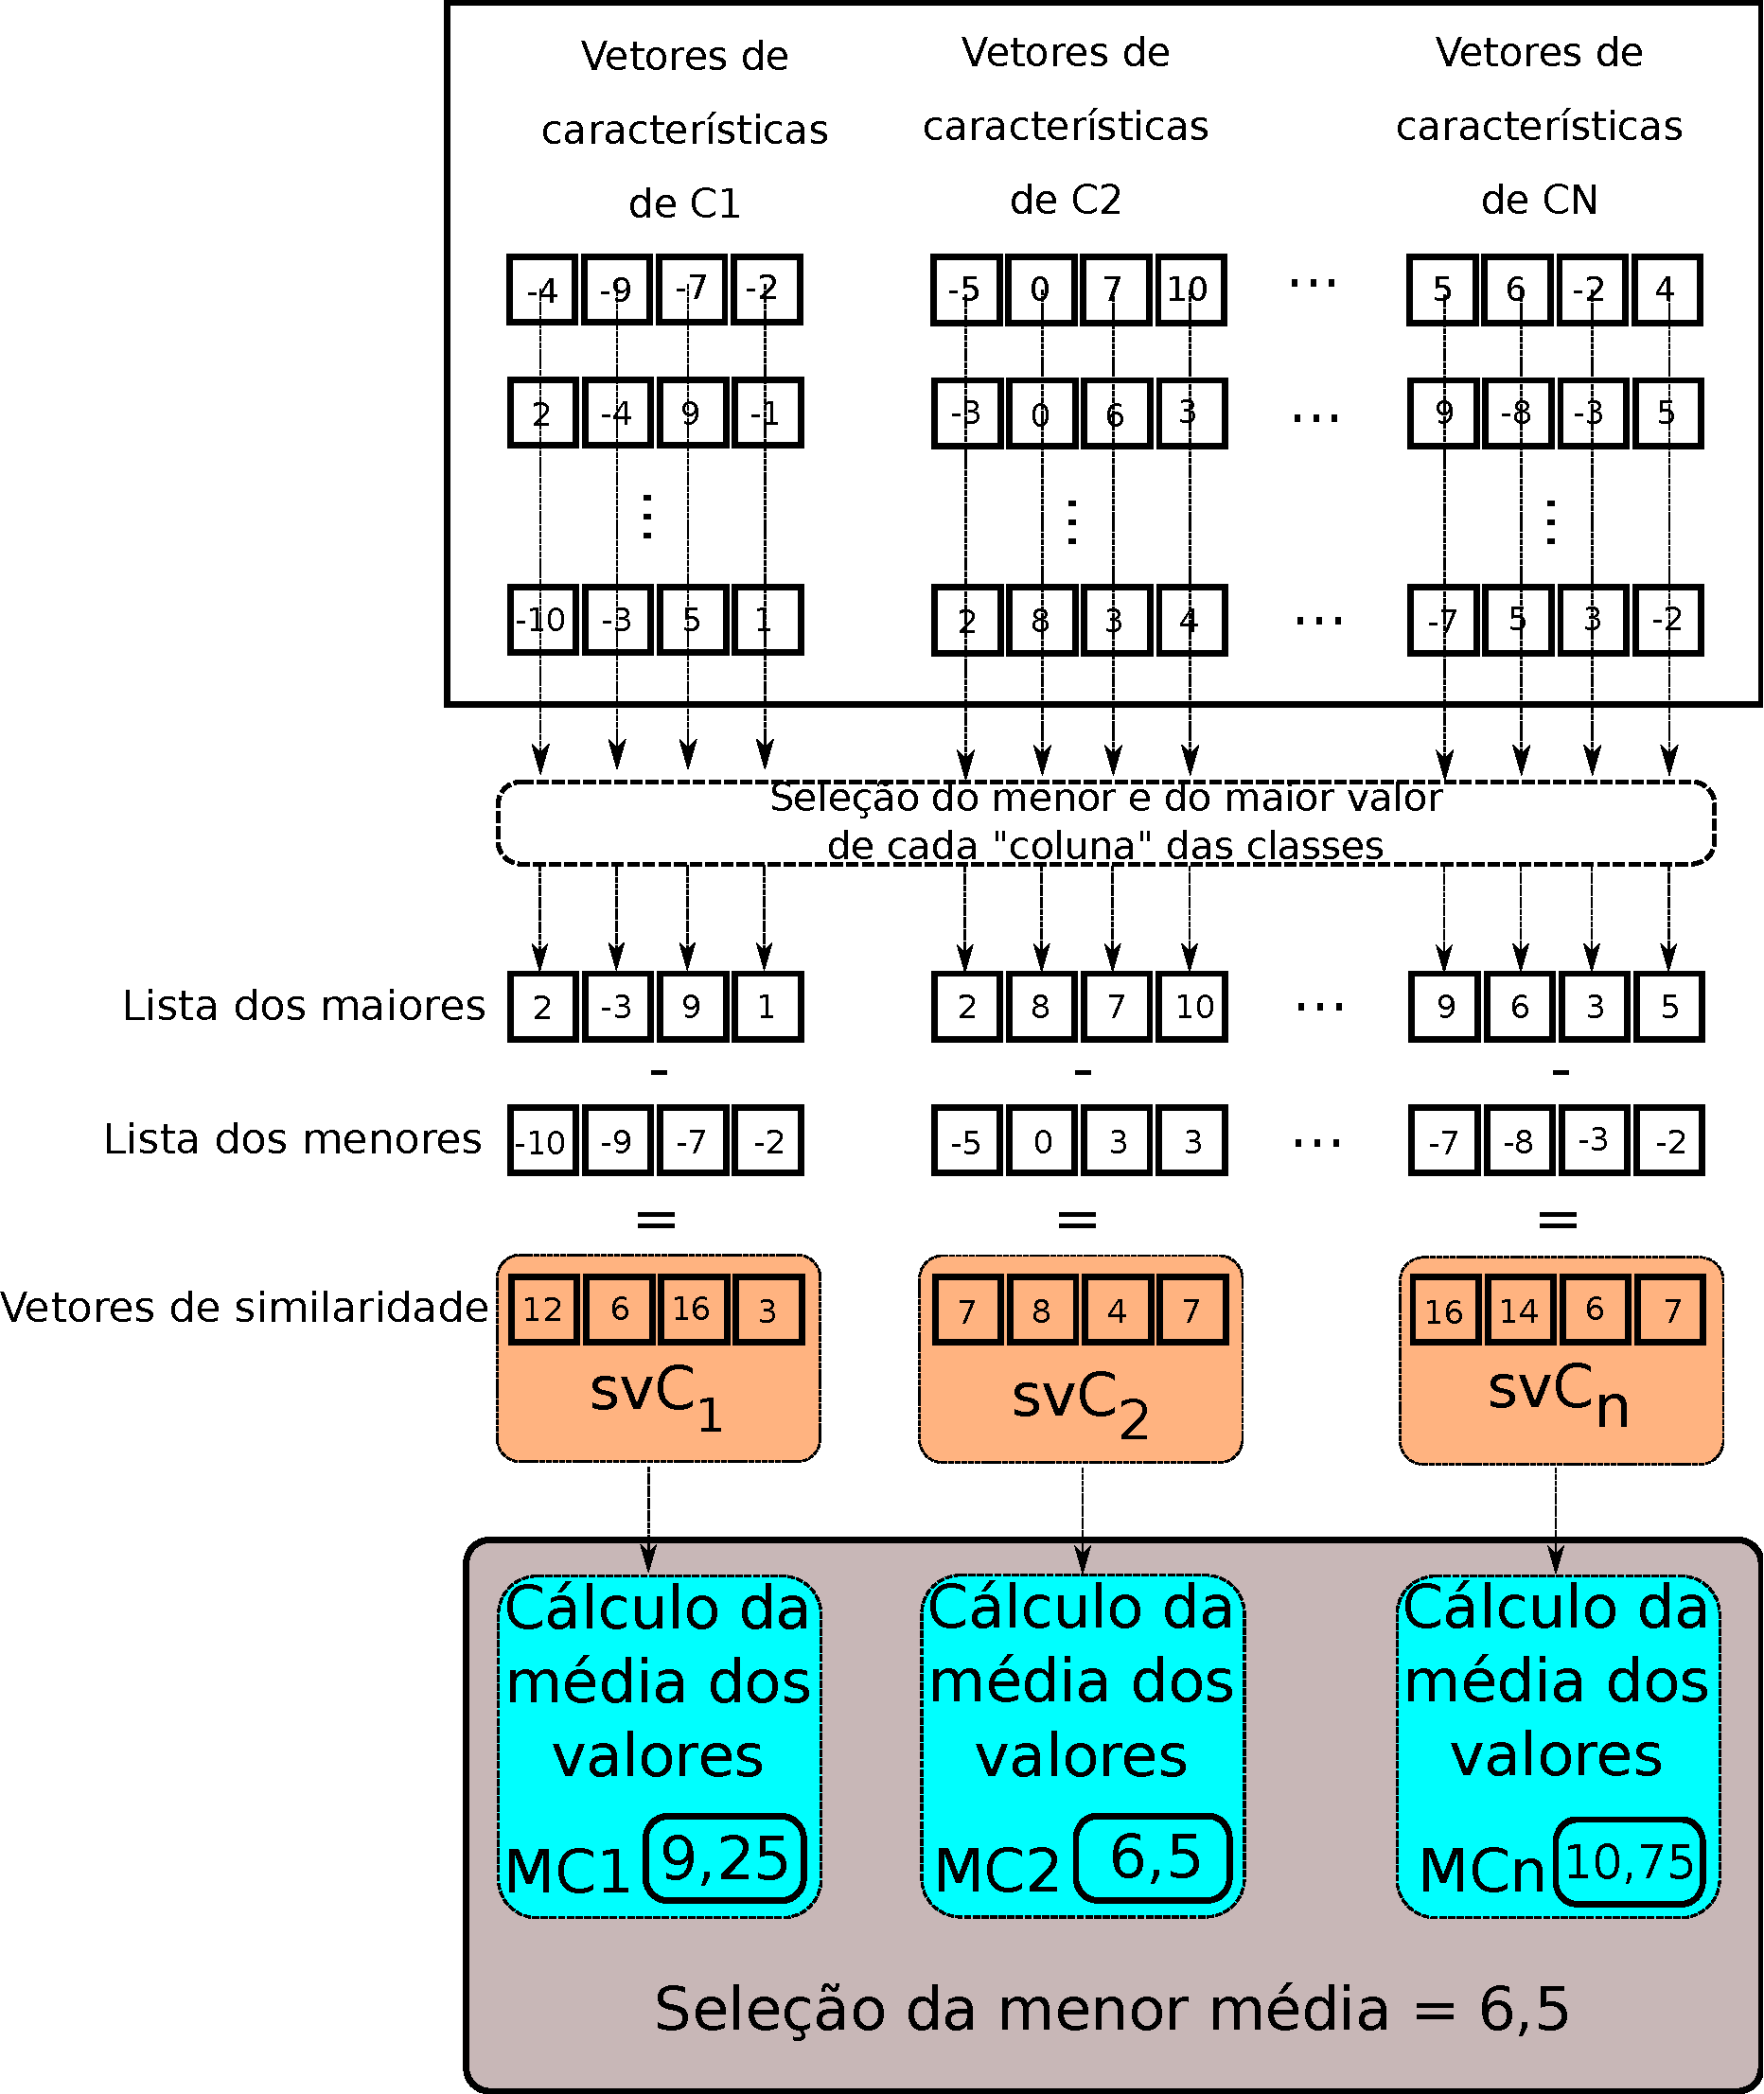
\includegraphics[width=0.5\linewidth]{images/calculoAlpha.pdf}
				\label{fig:calculoalpha}
				\\Fonte: Adaptado de \cite{8588433}.
			\end{figure}
			
			\par A obtenção de $\beta$, assim como ilustrado na Figura \ref{fig:betacalculation}, também se dá selecionando os maiores e os menores valores de cada uma das posições de todos os vetores de características de cada classe, gerando assim um vetor para os valores maiores e outro para os menores.
			
			\par Na sequência, realiza-se o cálculo de $R$ cujo valor é a quantidade de vezes que um valor do vetor de características de uma classe se encontra entre os valores maiores e menores de outra classe.
			
			\par Seja:
			\begin{itemize}
				\item N a quantidades de classes;
				\item X a quantidade de vetores de características por classe;
				\item T o tamanho do vetor de características.
			\end{itemize}
			
			\par Então, $F$, que é o número máximo de sobreposições possíveis entre classes, é dado por:
			\begin{equation}
				F=N.(N-1).X.T \qquad.
			\end{equation}
			\par Finalmente, $\beta$ é calculado da seguinte forma:
			\begin{equation}
				\beta=\dfrac{R}{F} \qquad.
			\end{equation}
	
			\par Neste ponto, é importante notar que $\alpha=1$ sugere fortemente que os vetores de características de cada classe são similares e representam suas respectivas classes precisamente. Complementarmente, $\beta=0$ sugere os vetores de características de classes diferentes não se sobrepõe \cite{8588433}.
			
			\begin{figure}[h]
				\centering
				\caption{Cálculo de $\beta$: Os itens destacados em azul e rosa são aqueles pertencentes a classe C1 e CN que se sobrepõe, em verde, a sobreposição é entre C1 e C2. Para cada sobreposição verificada soma-se 1 ao valor $R$. Essa comparação é feita para todos os vetores de características de cada uma das classes.}
				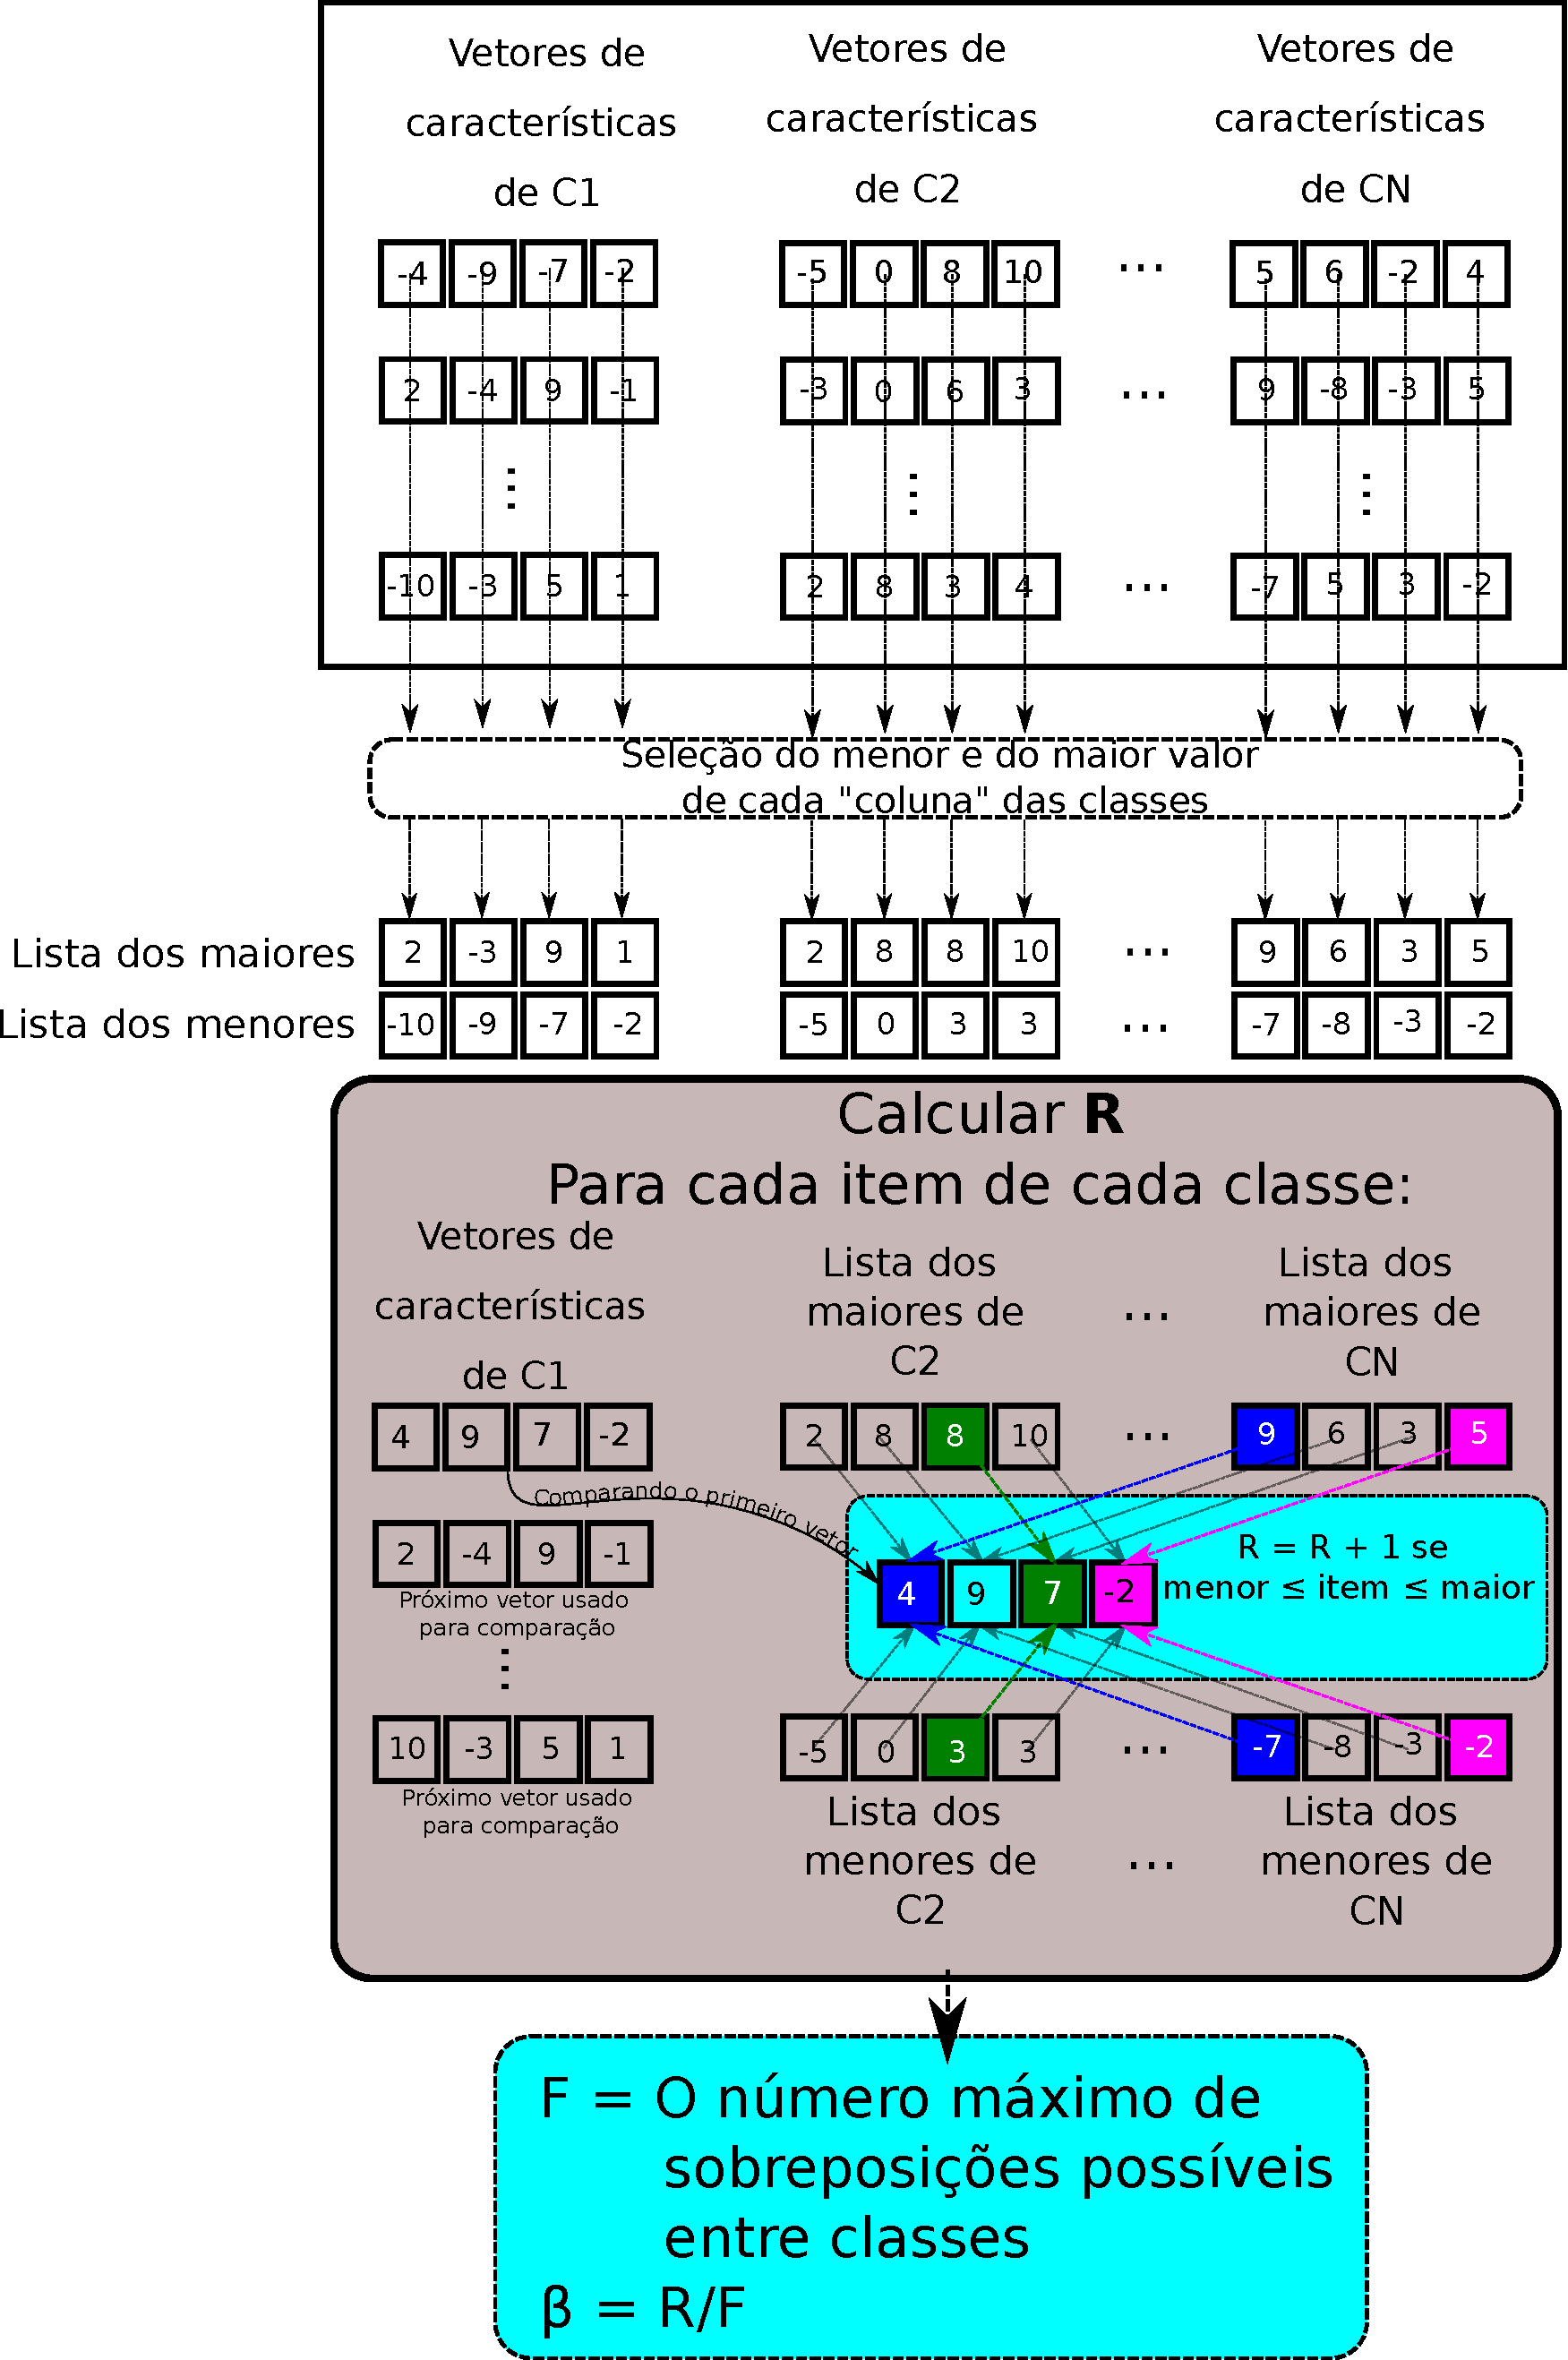
\includegraphics[width=0.5\linewidth]{images/betaCalculation.pdf}
				\label{fig:betacalculation}
				\\Fonte: Adaptado de \cite{8588433}.
			\end{figure}
			
			\par Considerando-se o plano paraconsistente \cite{8588433}, temos: 
			
			\begin{itemize}
				\item Verdade $\rightarrow$ fé total ($\alpha = 1$) e nenhum descrédito ($\beta = 0$)
				\item Ambiguidade $\rightarrow$ fé total ($\alpha = 1$) e descrédito total ($\beta = 1$)
				\item Falsidade $\rightarrow$ fé nula ($\alpha = 0$) e descrédito total ($\beta = 1$)
				\item Indefinição $\rightarrow$ fé nula ($\alpha = 0$) e nenhum descrédito ($\beta = 0$) \qquad.
			\end{itemize}
	
			\par No entanto, raramente $\alpha$ e $\beta$ terão valores inteiros como os mostrados na listagem acima: Na maioria das ocasiões, $0 \leqslant \alpha \leqslant 1$ e $0 \leqslant \beta \leqslant 1$. Por isso, se torna necessário o cálculo do \textbf{grau de certeza}, isto é, $G_1$, e do \textbf{grau de contradição}, isto é, $G_2$, conforme segue:
			\begin{equation}
				G_1=\alpha-\beta  \qquad,
			\end{equation}
			\begin{equation}
				G_2=\alpha+\beta-1 \qquad,
			\end{equation}
			onde: $-1 \leqslant G_1$ e  $1 \geqslant G_2$.
			
			\par Os valores de $G_1$ e $G_2$, em conjunto, definem os graus entre verdade ($G_1=1$) e falsidade ($G_1=-1$) e também os graus entre indefinição ($G_2=-1$) e ambiguidade ($G_2=1$). Novamente, raramente tais valores inteiros serão alcançados já que $G_1$ e $G_2$ dependem de $\alpha$ e $\beta$.
	
			\par O Plano Paraconsistente, para fins de visualização e maior rapidez na avaliação dos resultados, encontra-se ilustrado na Figura \ref{fig:paraconsistentplane} e tem quatro arestas precisamente definidas:
			\begin{itemize}
				\item (-1,0) $\rightarrow$ falsidade;
				\item (1,0) $\rightarrow$ verdade;
				\item (0,-1) $\rightarrow$ indefinição;
				\item (0,1) $\rightarrow$ ambiguidade.
			\end{itemize}
			\par A propósito de ilustração na Figura \ref{fig:paraconsistentplane}, é possível ver um pequeno círculo indicando os graus dos quatro casos listados.
			
			\par Para se ter ideia em que área exatamente se encontram as classes avaliadas, as distâncias $(D)$ do ponto $P=(G_1,G_2)$ até o limites supracitados podem ser computadas. Tais cálculos podem ser feitos da seguinte forma:
	
			\begin{equation}
				D_{-1,0}=\sqrt{(G_1+1)^2+(G_2)^2}\qquad,
			\end{equation}
			\begin{equation}
				D_{1,0}=\sqrt{(G_1-1)^2+(G_2)^2}\qquad,
			\end{equation}
			\begin{equation}
				D_{0,-1}=\sqrt{(G_1)^2+(G_2+1)^2}\qquad,		
			\end{equation}
			\begin{equation}
				D_{0,1}=\sqrt{(G_1)^2+(G_2-1)^2}\qquad.
			\end{equation}		
			
			\begin{figure}[H]
				\centering
				\caption{O plano paraconsistente: O pequeno círculo indica os graus de falsidade(-1,0), verdade(1,0), indefinição(0,-1) e ambiguidade(0,1)}
				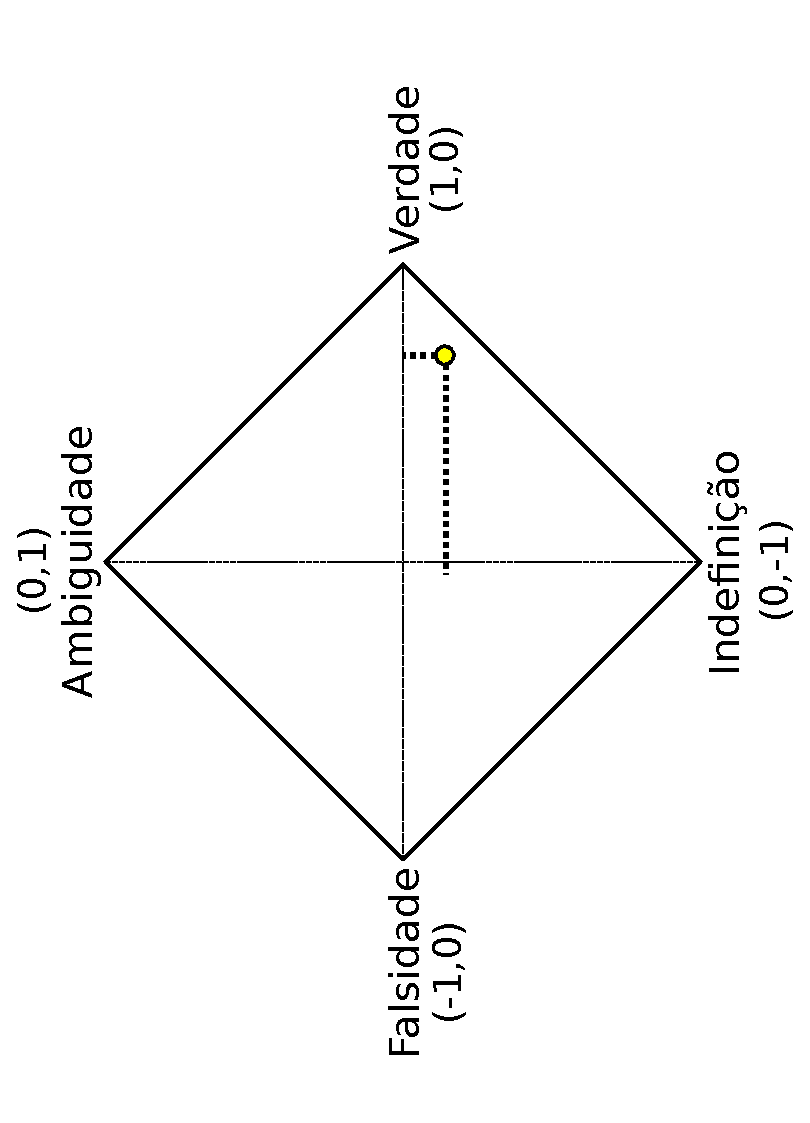
\includegraphics[angle=-90, width=0.69\linewidth]{images/paraconsistentPlane.pdf}
				\label{fig:paraconsistentplane}
				\\Fonte: Adaptado de \cite{8588433}.
			\end{figure}
			\par Na prática, ou seja, para fins de classificação, geralmente considera-se a distância em relação ao ponto \textit{``(1,0) $\rightarrow$ Verdade''}, que é o ponto ótimo: quanto mais próximo o ponto $(G_1,G_2)$ estiver de $(1,0)$, mais as os vetores de características das diferentes classes estão naturalmente separados. Isso implica, dentro da limitação de cada algoritmo, em resultados melhores sejam quais forem os classificadores usados.
	
	\subsection{Brain-Computer Interface and EEG}
		\par Among the methods of Brain-Computer Interface (BCI), Electroencephalogram (EEG) stands out as the most cost-effective and simple system to implement. However, it does have some quirks, such as high sensitivity to electromagnetic interference and difficulty in capturing the signal due to suboptimal scalp placement of the electrodes. So one of the fundamental aspects that any EEG processing system must have is the tolerance to noise \cite{JALALYBIDGOLY2020101788}.
		
		\par The \textit{wet} electrodes are placed using conductive gel and are less prone to movement artifacts which are electromagnetic interferences caused by some motion like blinking. \textit{Dry} electrodes do not need the gel but is more sensible to artifacts.
		
		\par EEG records the electrical activities of the brain, typically placing along the scalp surface electrodes. These electrical activities result from ionic current flows induced by the synchronized synaptic activation of the brain's neurons. They manifest as rhythmic voltage fluctuations ranging from 5 to 100$\mu V$ in amplitude and between 0.5 and 40 Hz in frequency\cite{JALALYBIDGOLY2020101788}. The operational frequencies bands in the brain are following \cite{sanei2021eeg}:
		
		\begin{itemize}
			\item \textbf{Delta (1–4Hz)}: The slowest and usually the highest amplitude waveform. The Delta band is observed in babies and during deep sleep in adults.
			
			\item \textbf{Theta (4–8Hz)}: Observed in children, drowsy adults, and during memory recall. Theta wave amplitude is typically less than 100$\mu V$.
			
			\item \textbf{Alpha (8–12Hz)}: Usually the dominant frequency band, appearing during relaxed awareness or when eyes are closed. Focused attention or relaxation with open eyes reduces the amplitude of the Alpha band. These waves are normally less than 50 $\mu V$.
			
			\item \textbf{Beta (12–25Hz)}: Associated with thinking, active concentration, and focused attention. Beta wave amplitude is normally less than 30 $\mu V$.
			
			\item \textbf{Gamma (over 25Hz)}: Observed during multiple sensory processing. Gamma patterns have the lowest amplitude.
		\end{itemize}
		
		\par According to \cite{JALALYBIDGOLY2020101788}, for most of the tasks brain do, there are regions associated with it as seen in Table \ref{tb:brainRegions}.
		
		
		\subsection{10-20 system and the brain's areas}
		\begin{table}[H]
			\begin{center}
				\caption{Brain tasks and its corresponding regions. See Figure \ref{fig:1020standardandlobes} for more information.}
				\begin{tabular}{|c|c|p{0.4\textwidth}|}
					\hline
					Region & Channels & Tasks\\
					\hline
					Frontal lobe & Fp1, Fp2, Fpz, Pz, F3, F7, F4, F8 & Memory, concentration, emotions.\\
					\hline
					Parietal lobe& P3, P4, Pz & Problem Solving, attention, grammar, sense of touch. \\
					\hline
					Temporal lobe& T3, T5, T4, T6 & Memory, recognition of faces, hearing, word and social clues. \\
					\hline
					Occipital lobe & O1, O2, Oz & Reading, vision.\\
					\hline
					Cerebellum && Motor control, balance. \\
					\hline
					Sensorimotor Cortex & C3, C4, Cz& Attention, mental processing, fine motor control, sensory integration. \\
					\hline
				\end{tabular}
				\label{tb:brainRegions}
			\end{center}
		\end{table}
		
		\begin{figure}[H]
			\centering
			\includegraphics[width=0.8\linewidth]{images/10–20StandardAndLobes}
			\caption[10-20 standard and brain lobes]{Electrodes placement according to 10-20 standard \cite{sistema10-20} and brain's lobes. Odd numbers are assigned to the electrodes on the left hemisphere, and even numbers are assigned to the electrodes on the right. Source \cite{JALALYBIDGOLY2020101788}}
			\label{fig:1020standardandlobes}
		\end{figure}
	
	\subsection{Spiking Neural Networks}
		\par Neural Networks (NNs), as defined here as \textit{a multilayered, fully connected, with or without recurrent or convolutional layers network}, require that all neurons are activated in both the forward and backward passes. This implies that every unit in the network must process some data, leading to power consumption \cite{10242251}. 
		
		\par The sensory system of biological neurological systems converts external data, such as light, odors, touch, flavors, and others, into \textbf{spikes}. A spike is a voltage that convey information \cite{kasabov2019time}. These ones are then transmitted along the neuronal chain to be processed, generating a response to the environment.
		
		\par The biological neuron only spikes when a certain level of excitatory signals get accumulated above some threshold in its soma staying inactive when there is no signal, therefore, this type of cell is very efficient in terms of energy consumption and processing.
		
		\par In order to get the aforementioned advantages the Spiking Neural Networks (SNNs) instead of employing continuous activation values, like NNs, SNNs utilize \textbf{spikes} at the input, hidden and outputs layers. SNNs can have continuous inputs as well and keep its properties.
		
		
		\par A SNN \textbf{is not} a one-to-one simulation of neurons. Instead, it approximates certain computational capabilities of specific biological properties. Some studies like \cite{jones2020single} created models way closer to natural neurons exploring the nonlinearity of dendrites and another neuron features yielding remarkable results in the classification.
		
		\par As can be seen in Figure \ref{fig:neuronspike} SNNs neurons, given the correct parameters, are very noise tolerant because it acts as a \textbf{lowpass filter}. Generating spikes even when a considerably level of interference is present. This units are very time-oriented too, being great when it comes to process streams of data \cite{10242251}.
		
		\begin{figure}[H]
			\centering
			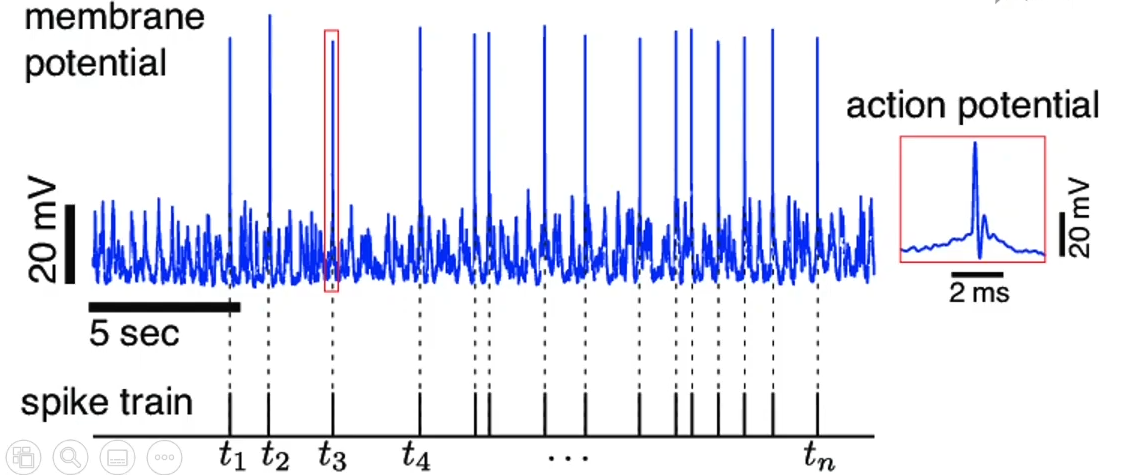
\includegraphics[width=\linewidth]{images/neuronSpikes}
			\caption{Spikes from a noisy signal. Source \cite{dan_goodman_2022_7044500}}
			\label{fig:neuronspike}
		\end{figure} 
		
		\subsection{Spiking Neuron}
		\par Although the focus of this work is the \textit{Leaky Integrate and Fire Neurons} (LIF) because is simpler, more efficient and currently generalize better for most of the problems \cite{dan_goodman_2022_7044500}, there are more biological accurate model like \textbf{Hodgkin-Huxley neuron} \cite{gerstner2014neuronal} and ones like \cite{jones2020single} that created models closer to natural neurons exploring the nonlinearity of dendrites and other neuron features.
		
		\subsubsection{Leaky Integrate and Fire Neuron}
		\par The Leaky Integrate and Fire Neuron (LIF) is one of the simplest neuron models in SNNs, still, it can be applied successfully to most of the problems in with SNNs can be used.
		
		\par LIF, like a NN neuron takes the sum of weighted inputs but, rather than pass it directly to its activation function, some \textit{leakage} is applied, which decreases in some degree the sum. 
		\par LIF behave much like Resistor-Capacitor circuits as can be seen in Figure \ref{fig:rcmodel}. Here $R$ is resistance to the leakage, $I_{in}$ the input current, $C$ the capacitance, $U_{mem}$ means the accumulated action potential and $v$ is a switch that lets the capacitor discharge (i.e. emit a spike) when some potential threshold is reached.
		
		\begin{figure}[H]
			\centering
			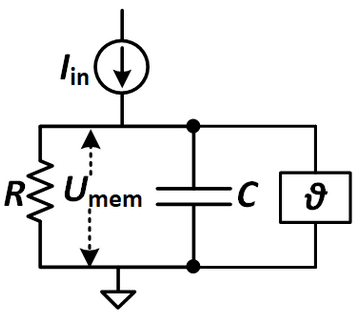
\includegraphics[width=0.4\linewidth]{images/rcmodel}
			\caption[The RC model]{RC model: Source: \cite{10242251}}
			\label{fig:rcmodel}
		\end{figure}
		
		\par Unlike the Hodgkin-Huxley neuron, spikes are represented as \textbf{sparsely} distributed \textbf{ones} in a train of \textbf{zeros}, as illustrated in Figure \ref{fig:spikessparsitystaticsupress} and \ref{fig:sparsity}. This approach simplify the models and reduces the computational power and needed storage to run a SNN.\newline
		
		\begin{figure}[H]
			\centering
			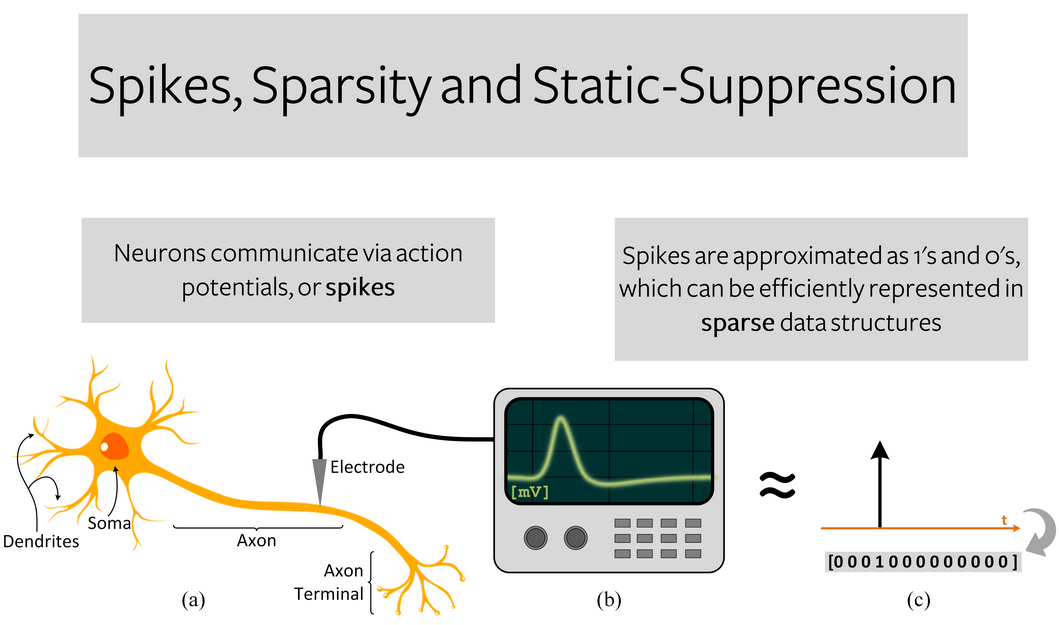
\includegraphics[width=\linewidth]{images/spikesSparsityStaticSupress}
			\caption{Sparsity on Spike Neuron Networks. Source: \cite{10242251}}
			\label{fig:spikessparsitystaticsupress}
		\end{figure}
		
		\begin{figure}[H]
			\centering
			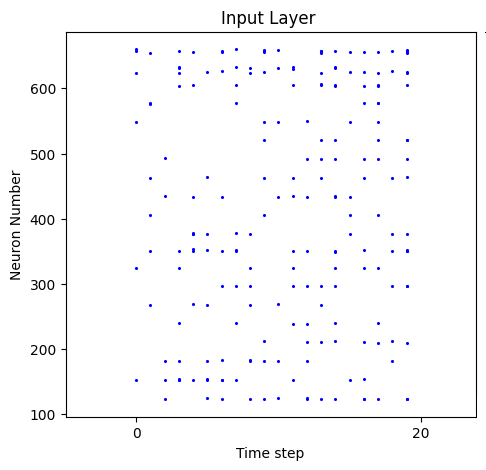
\includegraphics[width=.5\linewidth]{images/sparsity}
			\caption[Sparse activity of a SNN]{Sparse activity of a SNN: The horizontal axis represents the time step of some data being processed the vertical are the SNN neuron number. Note that, most of the time, very few neurons gets activated. Source: The author.}
			\label{fig:sparsity}
		\end{figure}
		
		\par As result of the mentioned above, in SNN information is coded in format of \textit{timing} and/or \textit{rate} of spikes giving consequently great capabilities of processing streams of data but limiting the processing of static data.\newline
		
		\par LIF model is governed by the Equations bellow \cite{10242251}.
		
		
		\par Considering that $Q$ is a measurement of electrical charge and $V_{mem}(t)$ is the potential difference at the membrane in a certain time $t$ than the neuron capacitance $C$ is given by the Equation \ref{eq:capacitance}.
		
		\begin{equation}
			\label{eq:capacitance}
			C = \frac{Q}{V_{mem}(t)}
		\end{equation}
		
		\par Than the neuron charge can be expressed as Equation \ref{eq:charge}.
		
		\begin{equation}
			\label{eq:charge}
			Q = C.V_{mem}(t)
		\end{equation}
		
		\par To know how these charge changes according to the time (aka current) we can derivate $Q$ as in Equation \ref{eq:rateOfChargeChange}. This expression express the current in the capacitive part of the neuron $I_C$
		
		\begin{equation}
			\label{eq:rateOfChargeChange}
			I_C = \dfrac{dQ}{dt} = C. \dfrac{dV_{mem}(t)}{dt}
		\end{equation}
		
		
		\par To calculate the total current passing by the resistive part of the circuit we may use the Ohm's law:
		
		\begin{equation}
			\label{eq:ohmlaw}
			V_{mem}(t) = R.I_R \implies I_R = \frac{V_{mem}(t)}{R}
		\end{equation}
		
		\par Than considering that the total current do not change, as seen in Figure \ref{fig:rcmodel2}, we have the total input current $I_{in}$ of the neuron as in Equation \ref{eq:totalNeuronCurrent}.
		
		\begin{figure}[H]
			\centering
			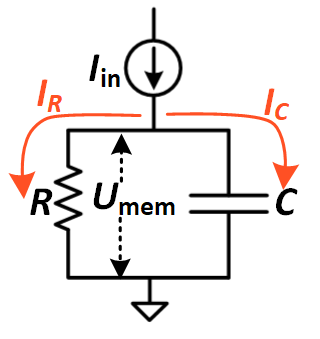
\includegraphics[width=0.4\linewidth]{images/rcmodel2}
			\caption[RC model for currents]{RC model for currents: $I_{in} = I_R + I_C$}
			\label{fig:rcmodel2}
		\end{figure}
		
		\begin{equation}
			\label{eq:totalNeuronCurrent}
			I_{in}(t) = I_R + I_C \implies I_{in}(t) = \frac{V_{mem}(t)}{R} + C.\dfrac{dV_{mem}(t)}{dt}
		\end{equation}
		\par Therefore, to describe the passive membrane we got a linear Equation \ref{eq:memLinear}.
		\begin{equation}
			\label{eq:memLinear}
			\begin{aligned}
				I_{in}(t) &= \frac{V_{mem}(t)}{R} + C.\dfrac{dV_{mem}(t)}{dt} \implies \\ 
				I_{in}(t) - \frac{V_{mem}(t)}{R} &=  C.\dfrac{dV_{mem}(t)}{dt} \implies \\
				\Aboxed{R.I_{in}(t) - V_{mem}(t) &=  R.C.\dfrac{dV_{mem}(t)}{dt}}
			\end{aligned}
		\end{equation}
		
		\par Than, if we consider $\tau = R.C$ as the \textbf{membrane time constant} we get voltages on both sides of Equation \ref{eq:finalMem} which \textbf{describes the RC circuit}.
		
		\begin{equation}
			\label{eq:finalMem}
			\begin{aligned}
				R.I_{in}(t) - V_{mem}(t) &=  R.C.\dfrac{dV_{mem}(t)}{dt} \implies \\
				R.I_{in}(t) - V_{mem}(t) &=  \tau.\dfrac{dV_{mem}(t)}{dt} \implies \\
				\Aboxed{\tau.\dfrac{dV_{mem}(t)}{dt} &= R.I_{in}(t) - V_{mem}(t)}
			\end{aligned}
		\end{equation}
		
		\par From that, and setting $I_{in} = 0$ (i.e. no input) and considering $\tau = R.C$ is a constant and a starting voltage $V_{mem}(0)$ the neuron's voltage behavior can be modeled as an exponential curve as can be seen in Equation \ref{eq:expmembrane}.
		
		\begin{equation}
			\label{eq:expmembrane}
			\begin{aligned}
				\tau.\dfrac{dV_{mem}(t)}{dt} &= R.I_{in}(t) - V_{mem}(t) \implies \\
				\tau.\dfrac{dV_{mem}(t)}{dt} &= -V_{mem}(t) = \\
				e^{\ln(V_{mem}(t))} &= e^{-\frac{t}{\tau}} = \\
				\Aboxed{V_{mem}(t) &= V_{mem}(0).e^{-\frac{t}{\tau}}}
			\end{aligned}
		\end{equation}
		
		\par Then one can say that: In the absence of an input $I_{in}$, the membrane potential decays exponentially as illustrated in Figure \ref{fig:membranepotentialdecay} and implemented in Listing \ref{lst:membranepotentialdecay}.
		
		\begin{lstlisting}[language=Python, caption={Python implementation of the action potential decaying of a LIF: $I_{in} = 0$}, label={lst:membranepotentialdecay}]
def lif(V_mem, dt=1, I_in=0, R=5, C=1):
	tau = R*C
	V_mem = V_mem + (dt/tau)*(-V_mem + I_in*R)
	return V_mem
\end{lstlisting}
		
		\begin{figure}[H]
			\centering
			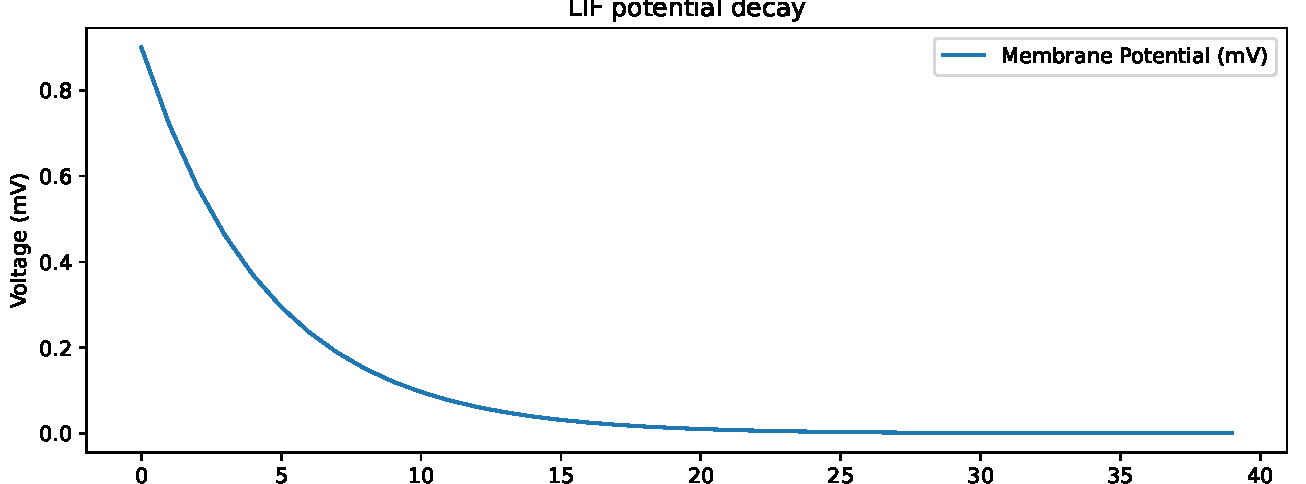
\includegraphics[width=\linewidth]{images/membranePotentialDecay}
			\caption{Membrane potential decaying. Source: The author}
			\label{fig:membranepotentialdecay}
		\end{figure}
		
		\par With the results from Equation \ref{eq:finalMem} it is possible to calculate the action potential increasing as seen in Equation \ref{eq:actionpotincrease}.
		
		\begin{equation}
			\label{eq:actionpotincrease}
			\begin{aligned}
				&\tau.\dfrac{dV_{mem}(t)}{dt} = R.I_{in}(t) - V_{mem}(t) = \\
				&\dfrac{dV_{mem}(t)}{dt} + \frac{V_{mem}(t)}{\tau} = \frac{R.I_{in}(t)}{\tau} \implies \\
				&\text{Integrating factor: } e^{\int \frac{1}{\tau} dt} = e^{\frac{1}{\tau}.t} \implies \\
				&(e^{\frac{1}{\tau}.t}.V_{mem}(t))' = \frac{R.I_{in}(t)}{\tau}.e^{\frac{1}{\tau}.t} = \\
				&\int (e^{\frac{1}{\tau}.t}.V_{mem}(t))' = \int \frac{R.I_{in}(t)}{\tau}.e^{\frac{1}{\tau}.t} dt = \\
				&e^{\frac{1}{\tau}.t}.V_{mem}(t) = \int \frac{R.I_{in}(t)}{\tau}.e^{\frac{1}{\tau}.t} dt \therefore \\
				& \text{Considering: } V_{mem}(t=0) = 0 \implies \\
				\Aboxed{&V_{mem}(t) = I_{in}(t).R(1-e^{\frac{1}{\tau}})}
			\end{aligned}
		\end{equation}
		
		\par Note that when action potentials increases there is still an exponential behavior as seen in Figure \ref{fig:membranepotentialincrease} and implemented in Listing \ref{lst:membranepotentialincrease}.
		
		\begin{lstlisting}[language=Python, caption={Python implementation of the action potential decreasing of a LIF: $I_{in}=1$}, label={lst:membranepotentialincrease}]
	
def lif(V_mem, dt=1, I_in=1, R=5, C=1):
	tau = R*C
	V_mem = V_mem + (dt/tau)*(-V_mem + I_in*R)
	return V_mem
\end{lstlisting}
		
		\begin{figure}[H]
			\centering
			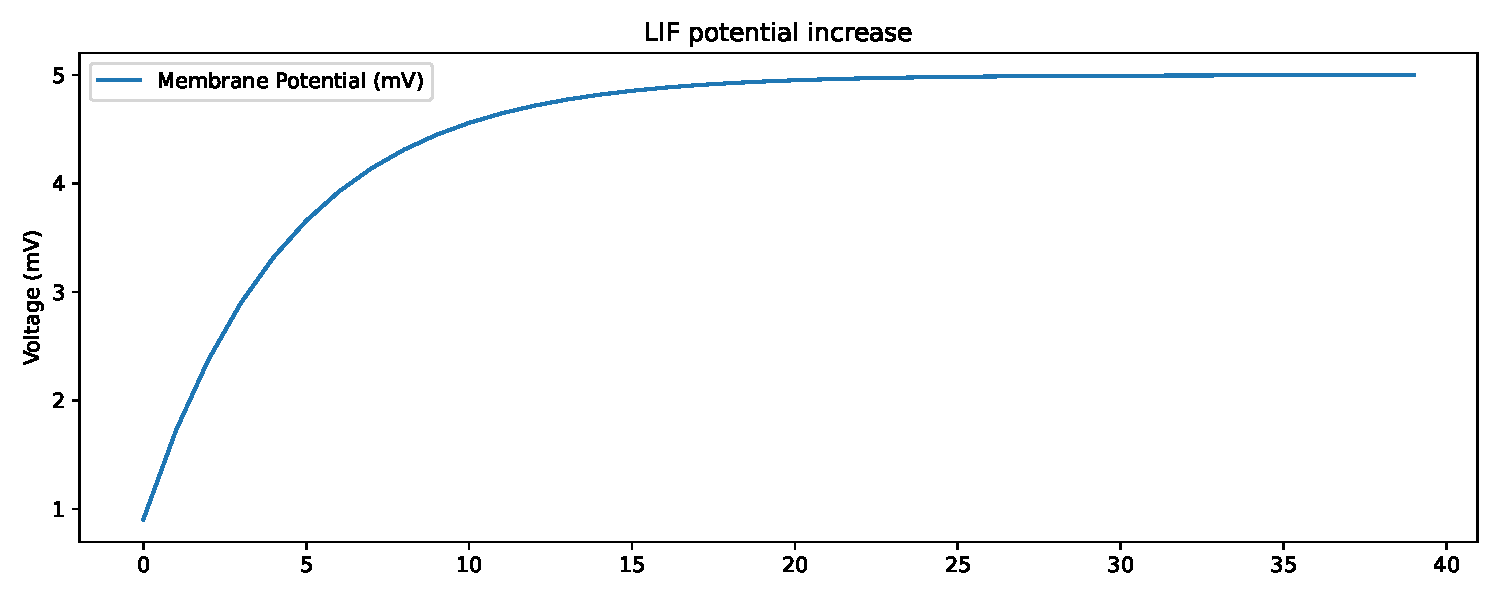
\includegraphics[width=\linewidth]{images/membranePotentialIncrease}
			\caption{Membrane potential increasing. Source: The author}
			\label{fig:membranepotentialincrease}
		\end{figure}
		
		\par Then taking into account some \textbf{threshold} which indicates a reset into the neuron potential and two type of resets (to zero and threshold subtraction) finally is possible to model the full LIF  behavior as depicted in Figure \ref{fig:membranepotentialfull} and implemented in Listing \ref{lst:membranepotentialfull}:
		
		\begin{lstlisting}[language=Python, caption={Python implementation of the action potential full simulation of a LIF: $I_{in}=1$, $V_{thresh} = 2$ is threshold}, label={lst:membranepotentialfull}]
def lif(V_mem, dt=1, I_in=1, R=5, C=1, V_thresh = 2, reset_zero = True):
	tau = R*C
	V_mem = V_mem + (dt/tau)*(-V_mem + I_in*R)
	if V_mem > V_thresh:
		if reset_zero:
			V_mem = 0
		else:
			V_mem = V_mem - V_thresh
	return V_mem
\end{lstlisting}

		
		\begin{figure}[H]
			\centering
			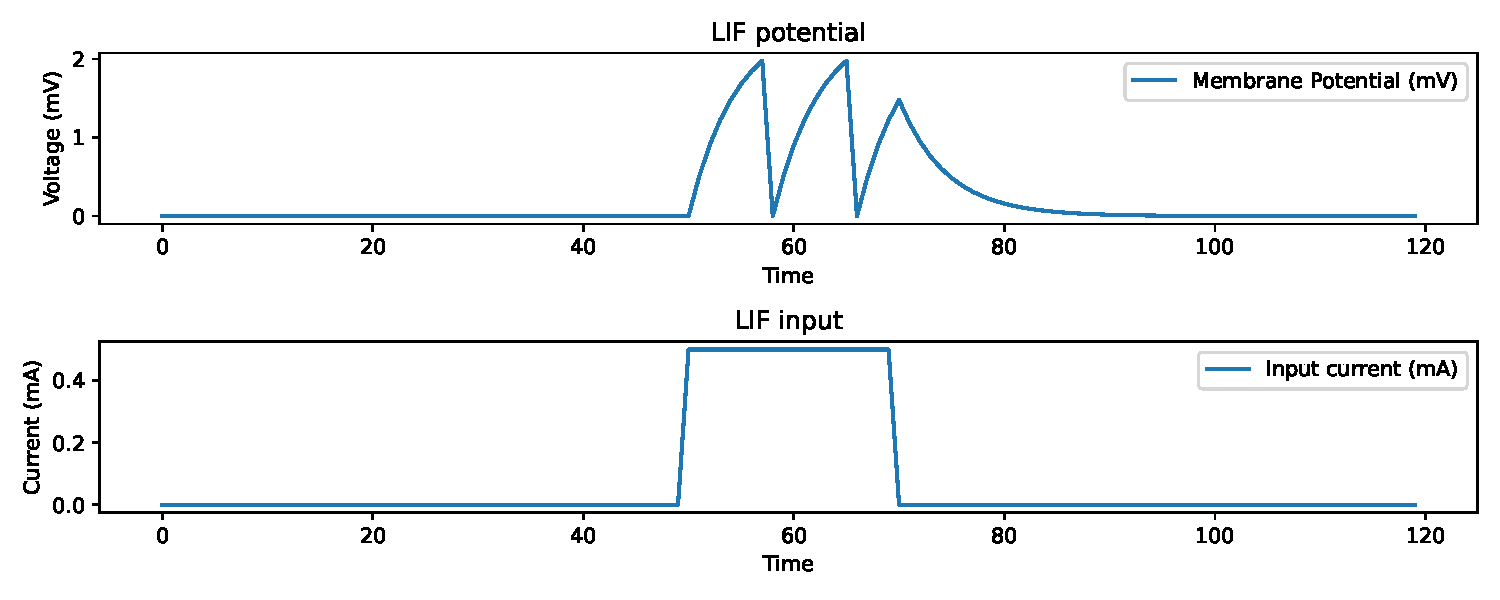
\includegraphics[width=\linewidth]{images/membranePotentialFull}
			\caption{Plot of the full simulated LIF: A 0.5 mA was provided from time 51 to 70.}
			\label{fig:membranepotentialfull}
		\end{figure}
		
		\subsection{Another interpretation of LIF}
		
			\par Starting with the Equation \ref{eq:finalMem} and using Forward Euler Method to solve the LIF model:
			
			\begin{equation}
				\tau.\dfrac{dV_{mem}(t)}{dt} = R.I_{in}(t) - V_{mem}(t)
			\end{equation}
			
			\par Solving the derivative in Equation \ref{eq:membraneDerivative} results in the membrane potential for any time $t+\Delta t$ in future:
			
			\begin{equation}
				\label{eq:membraneDerivative}
				\begin{aligned}
					\tau.\dfrac{V_{mem}(t+\Delta t) - V_{mem}(t)}{\Delta t} &= R.I_{in}(t) - V_{mem}(t) = \\
					V_{mem}(t+\Delta t) - V_{mem}(t) &= \frac{\Delta t}{\tau} . (R.I_{in}(t) - V_{mem}(t)) = \\
					\Aboxed{V_{mem}(t+\Delta t) &= V_{mem}(t) + \frac{\Delta t}{\tau} . (R.I_{in}(t) - V_{mem}(t))}
				\end{aligned}
			\end{equation}
	
		\subsection{Training}
		
		\par \textbf{How do SNNs get trained?} Well, this is still an open question. A SNN neuron has an activation-function behavior that is more relatable to a \textbf{step function}. Therefore, in principle, we can't use gradient descent-based solutions because this kind of function \textbf{is not} differentiable \cite{kasabov2019time}.
		
		\par But there are some insights out there that may shed some light on this subject: While some \textit{in vivo/in vitro} observations show that brains, in general, learn by strengthening/weakening and adding/removing synapses or even by creating new neurons or other cumbersome methods like RNA packets, there are some more acceptable ones like the ones in the list bellow \cite{kasabov2019time}:
		
		\begin{itemize}
			\item \textbf{Spike Timing-Dependent Plasticity (STDP)}: If a pre-synaptic neuron fires \textbf{before} the post-synaptic one, there is a strengthening in connection, but if the post-synaptic neuron fires before, then there is a weakening.
			\item \textbf{Surrogate Gradient Descent}: Approximates the step function by using another mathematical function, which is differentiable (like a sigmoid), in order to train the network. These approximations are used only in the backward pass, while keeping the step function in the forward pass \cite{kasabov2019time}.
			\item \textbf{Evolving Algorithms}: Use the selection of the fittest throughout many generations of networks.
			\item \textbf{Reservoir/Dynamic Computing}: \textbf{Echo state networks} or \textbf{Liquid state machines} respectively.
		\end{itemize}
		
		\par The one used in the SNN made in this work were \textbf{Surrogate Gradient Descent}.
	
		\subsection{Autoencoders}
		
			\par Como ilustrado na Figura \ref{fig:autoencoder} \textit{Autoencoders} são redes neurais treinadas para reconstruir seus dados de entrada. Eles consistem em uma função codificadora, denotada como $h = f(x)$, e uma função decodificadora que produz uma reconstrução, denotada como $r = g(h)$. A camada oculta $h$ representa um código ou representação comprimida da entrada \cite{Goodfellow-et-al-2016}. \newline
			
			\par O principal objetivo de um \textit{autoencoder} é aprender uma representação compactada dos dados de entrada na camada oculta e, em seguida, reconstruir os dados de entrada com a maior precisão possível usando o decodificador. No entanto, os \textit{autoencoders} são projetados para serem incapazes de copiar perfeitamente os dados de entrada. Eles geralmente são limitados de alguma forma para apenas aproximar a entrada e priorizar certos aspectos dos dados. \newline
			
			\par \textit{Autoencoders} podem ser treinados usando várias técnicas, como \textit{gradient descent} com \textit{minibatch} ou estocástico \cite{Goodfellow-et-al-2016}.
	
			\begin{figure}[h]
				\centering
				\caption[autoencoder]{\textit{Autoencoder}: $x$ é codificado para uma dimensão menor $h$ e, em seguida, é reconstruído em $r$, tal processo pode implicar ou não em uma perda na reconstrução}
				\begin{tikzpicture}[node distance=1.5cm, every edge/.style={draw=black,->}]
	% Nodes
	\node[draw, circle] (x) {$x$};
	\node[draw, rectangle, above right=0.7cm and 1cm of x] (encoder) {Codificador};
	\node[draw, circle, above right=0.7cm and 1cm of encoder] (h) {$h$};
	\node[draw, rectangle, below right=0.7cm and 1cm of h] (decoder) {Decodificador};
	\node[draw, circle, below right=0.7cm and 1cm of decoder] (r) {$r$};
	
	% Arrows
	\draw (x) edge (encoder);
	\draw (encoder) edge (h);
	\draw (h) edge (decoder);
	\draw (decoder) edge (r);
	
	% Loss
	\node[below of=h, yshift=-0.7cm] (loss) {Perda na reconstrução};
	\draw (x) edge (loss);
	\draw (r) edge (loss);
	
	% Labels
	\node[below of=x, yshift=0.7cm] {Entrada};
	\node[below right=0.2cm and 0.8cm of decoder] {Saída};
	\node[below of=r, yshift=0.7cm] {Entrada reconstruida};
\end{tikzpicture}
				\label{fig:autoencoder}
			\end{figure}
			
			\par Considerando-se que a reconstrução $r$ seja razoável, isso significa que a região $h$  contém dados suficientes para representar a informação em sua essência, sendo assim, dentro do contexto das redes neurais, autoencoders são ótimos produtores de vetores de características.
	
		\subsection{Redes neurais residuais (ResNets)}
			\par Segundo \cite{DBLP:journals/corr/HeZRS15} a ideia-chave por trás do \textit{ResNets} é a inclusão de conexões de salto como ilustrado na Figura \ref{fig:residualblock}, também conhecidas como mapeamentos de identidade, que permitem que a saída de uma camada seja adicionada diretamente à entrada da camada subsequente. Isso contorna as camadas intermediárias e garante que redes mais profundas possam aprender. Outra vantagem no uso de conexões de salto é que essa prática diminui a ocorrência de \textit{vanishing gradients} um problema comum em redes com muitas camadas que pode impossibilitar ou diminuir a níveis impraticáveis o aprendizado da rede.
			
			\begin{figure}
				\centering
				\caption[bloco de uma Resnet]{Bloco de uma Rede Neural Residual, $X$ é uma função identidade que contorna as camada intermediárias criando "\textit{highway connections}"}
				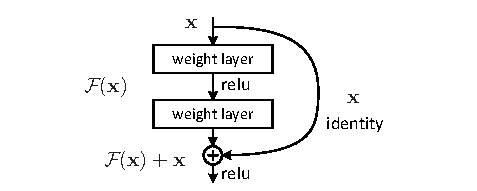
\includegraphics[width=0.7\linewidth]{images/residualBlock}
				\\ Fonte: \cite{DBLP:journals/corr/HeZRS15}
				\label{fig:residualblock}
			\end{figure}